%%
%% This is file `thesis.tex',
%% generated with the docstrip utility.
%%
%% The original source files were:
%%
%% nudtpaper.dtx  (with options: `thesis')
%% 
%% This is a generated file.
%% 
%% Copyright (C) 2018 by Liu Benyuan <liubenyuan@gmail.com>
%% 
%% This file may be distributed and/or modified under the
%% conditions of the LaTeX Project Public License, either version 1.3a
%% of this license or (at your option) any later version.
%% The latest version of this license is in:
%% 
%% http://www.latex-project.org/lppl.txt
%% 
%% and version 1.3a or later is part of all distributions of LaTeX
%% version 2004/10/01 or later.
%% 
%% To produce the documentation run the original source files ending with `.dtx'
%% through LaTeX.
%% 
%% Any Suggestions : LiuBenYuan <liubenyuan@gmail.com>
%% Thanks Xue Ruini <xueruini@gmail.com> for the thuthesis class!
%% Thanks sofoot for the original NUDT paper class!
%% 
%1. 规范硕士导言
% \documentclass[master,ttf]{nudtpaper}
%2. 规范博士导言
% \documentclass[doctor,twoside,ttf]{nudtpaper}
%3. 建议使用OTF字体获得较好的页面显示效果
%   OTF字体从网上获得,各个系统名称统一。
%   如果你下载的是最新的(1201)OTF英文字体,建议修改nudtpaper.cls,使用
%   Times New Roman PS Std
% \documentclass[doctor,twoside,otf]{nudtpaper}
%   另外,新版的论文模板提供了方正字体选项FZ,效果也不错哦
% \documentclass[doctor,twoside,fz]{nudtpaper}
%4. 如果想生成盲评,传递anon即可,仍需修改个人成果部分
% \documentclass[master,otf,anon]{nudtpaper}
%
\documentclass[master,otf]{nudtpaper}
\usepackage{mynudt}

\classification{TP391}
\serialno{16063284}
\confidentiality{公开}
\UDC{004.8}
\title{分布式深度学习系统中低精度数据\\同步技术的研究与实现}
\displaytitle{分布式深度学习系统中低精度数据同步技术的研究与实现}
\author{陈晓涛}
\zhdate{\zhtoday}
\entitle{A Research of Low Precision Data Synchronization Technology on Distributed Deep Learning System}
\enauthor{Chen Xiaotao}
\endate{\entoday}
\subject{集成电路专业}
\ensubject{Integrated Circuits}
\researchfield{分布式深度学习}
\supervisor{李东升\quad{}研究员}
\cosupervisor{张钊宁\quad{}助理研究员} % 没有就空着
\ensupervisor{Prof. Li Dongsheng}
\encosupervisor{Assistant Prof. Zhang Zhaoning} % 没有就空着
\papertype{专业学位}
\enpapertype{Engineering}
% 加入makenomenclature命令可用nomencl制作符号列表。

\begin{document}
\graphicspath{{figures/}}
% 制作封面,生成目录,插入摘要,插入符号列表 \\
% 默认符号列表使用denotation.tex,如果要使用nomencl \\
% 需要注释掉denotation,并取消下面两个命令的注释。 \\
% cleardoublepage% \\
% printnomenclature% \\
\maketitle
\frontmatter
\tableofcontents
\listoftables
\listoffigures

\midmatter
\begin{cabstract}
近年来以神经网络为基础的人工智能技术在学术界和工业界得到了广泛应用和发展。随着神经网络模型和训练所需的数据量不断增加,使得单机训练神经网络越来越困难。分布式训练神经网络不仅可以极大减少训练时间,也可对某些单机情况下无法训练的神经网络进行训练。在可预见的未来,分布式训练神经网络将成为必然选择。如何提高分布式训练神经网络的效率和可扩展性则显得尤为重要。

本文针对这一问题提出低精度分布式更新算法LPDU,将原始浮点数梯度转换为BF16格式进行传输,减少同步时间开销,进而提升分布式训练效率,通过混合精度更新算法,保证训练精度。本文通过分析LPDU算法各部分的时间开销和神经网络的参数规模得出LPDU算法在特定神经网络训练中的理论性能提升,并通过实验加以验证。通过对比LPDU算法与原始算法在图像分类,目标检测任务的相关实验,证明了LPDU算法在图像分类与目标检测任务中均能达到与原始更新算法相同的理想精度。同时对分布式训练性能有所提升。在8节点情况下,resnet50的训练效率由原始的84.05\%提升到了87.50\%,VGG网络的训练效率相对于原始的79.42\%提升至了86.55\%,SSD网络相对于原始效率有4.83\%的提升。

基于LPDU算法减少梯度尾数位的思路,本文提出两种极限精度梯度压缩方法EPGC:9比特梯度压缩方法和8比特梯度压缩方法。9比特梯度压缩方法是在浮点数基础上去除所有尾数位,仅使用1个符号位和8个指数位表示梯度;8比特梯度压缩方法是在半精度浮点数基础上去除8位尾数位,使用1个符号位,5个指数位和2个尾数位表示梯度。为快速验证本文提出的梯度压缩方法的可行性,本文通过在原始浮点数或半精度浮点数基础上对特定尾数位置零的方式模拟这两种压缩方法。通过实验证明这两种梯度压缩算法均能保证神经网络在图像分类任务中的训练精度,说明通过这两种梯度压缩算法提升分布式训练效率上可行的。

\end{cabstract}
\ckeywords{神经网络; 分布式训练; 低精度; 更新算法; 梯度压缩}

\begin{eabstract}
In recent years, the artificial intelligence technology based on neural networks has been widely used and developed in academia and industry. As neural network models and the amount of data required for training continue to increase, it becomes increasingly difficult to train neural networks in a single machine. The distributed training for neural networks not only greatly shorten the training time, but also provides a solution for some neural networks that cannot be trained in single machine. In the foreseeable future, the distributed training for neural networks will become an inevitable choice. How to improve the efficiency and scalability of distributed training for neural networks is particularly important.

This paper proposes a low-precision distributed update (LPDU) algorithm, which converts the original floating-point gradient into BF16 format for transmission, which reduces the synchronization time overhead and improves the efficiency of distributed training. The Mixed precision update  (MPU) algorithm can ensure the training accuracy. In this paper, by analyzing the time overhead in each part of LPDU algorithm and the parameter size of the neural network, the theoretical performance improvement of BF16 distributed update algorithm in specific neural network training is obtained and verified by experiments. By comparing the training accuracy curves between the LPDU algorithm and the original algorithm, it proves that the LPDU algorithm can achieve the same ideal precision as the original algorithm in both image classification and object detection tasks. And the efficiency of distributed training has improved. In the case of 8 nodes training, the efficiency of resnet50 has increased from the original 84.05 \% to 87.50\%. The training efficiency of the VGG has increased to 86.55\% compared with the original 79.42\%, and the SSD network has increased by 4.83\% compared with the original efficiency.

Based on the idea of LPDU algorithm that reduces the mantissa of gradient, two extreme precision gradient compression (EPGC) algorithms are proposed: 9-bits gradient compression algorithm and 8-bits gradient compression algorithm. The 9-bits gradient compression algorithm removes all mantissa bits in the float data format, only using 1 sign bit and 8 exponent bits to represent the gradient; the 8-bits gradient compression algorithm removes 8 bits in the mantissa of half-precision data. using 1 sign bit, 5 exponent bits and 2 mantissa bits represent the gradient. In order to quickly verify the feasibility of the two proposed gradient compression algorithms, this paper simulates the two compression algorithms by zeroing the specific mantissa position based on the original floating point number or half-precision floating point number. Experiments show that both gradient compression algorithms can guarantee the training accuracy of neural networks in image classification tasks. It is feasible to improve the efficiency of distributed training through these two gradient compression algorithms.

\end{eabstract}
\ekeywords{neural network; distributed training; low precision; update algorithm; gradient compression}


\input{data/denotation}

%书写正文,可以根据需要增添章节; 正文还包括致谢,参考文献与成果
\mainmatter
\chapter{绪论}
本章首先阐述了本课题的研究背景及现实意义,然后介绍国内外针对该问题的研究与进展。同时说明在实际应用中存在的问题和可进一步优化的方法。最后介绍本论文的整体组织结构。
\section{研究背景与意义}
近年来,以神经网络\upcite{alexnet2012}为代表的深度学习方法在图像处理、机器视觉、自然语言处理等诸多应用领域取得了巨大突破。自2012年AlexNet\upcite{alexnet2012}以绝对优势夺得ImageNet冠军后,神经网络逐渐得到学术界、工业界的广泛关注,开启了人工智能新篇章。随后各种性能更优、结构更复杂的网络如雨后春笋般层出不穷。如VGG、inception系列、resnet系列,denseNet等\upcite{vgg2014, inception2015, resnet2016, denselynet2017}。同时,鉴于卷积神经网络在图像分类领域的优异表现,业界将其应用到了目标检测、图像分割等领域。如fast rcnn系列\upcite{rcnn2014, fastrcnn2015, fasterrcnn2015}、yolo系列\upcite{yolo2016}、FPN\upcite{fpn2017}、R-FCN\upcite{rfcn2016}等。在自然语言处理领域,涌现出了一系列以循环神经网络[引用]为基础的深度学习方法,在机器翻译、文本分析、阅读理解等\upcite{gnmt2016, bert2018}问题上取得了显著进步,达到甚至超越人类水平。\\
因为神经网络参数量、计算量巨大,往往需要花费数天,乃至更长的时间。如最初的AlexNet\upcite{alexnet2012},需要5-6天训完。使得网络更新迭代设计周期变长,极大限制了科研人员的研究进度。随着网络结构复杂化迭代周期过长的问题尤为严重。分布式训练神经网络则能极大缩短训练周期,加速研究迭代、产品孵化等。同时,随着神经网络的不断发展以及社会对人工智能应用需求的提升,深度学习所需的数据量、网络模型也越来越大,单台计算机算力已经很难甚至无法满足其计算要求。为了减少神经网络的训练时间和适应不断增长的算力要求,分布式训练神经网络是必然选择。\\
本课题围绕着分布式训练神经网络的效率和精度进行展开,旨在保证网络性能前提下,提高分布式训练神经网络效率,提高训练加速比,缩短训练时间。本课题不仅能解决现今训练神经网络时间过长的问题, 更为今后单机场景下无法完成训练的神经网络提供了高效的训练方法。这对于现阶段和可预见未来都有重要实用价值,促进神经网络的发展,对人工智能的发展有深远意义。

\section{研究现状}
随着人工智能的快速发展,为提升训练效率,满足生产需求。业界已针对分布式深度学习系统进行了深入的研究。目前业界主流深度学习框架同时支持parameter servers和horovod进行分布式训练。如tensorflow,pytorch,mxnet等\upcite{tensorflow2016, torch2002, mxnet2015}均支持pamameter servers和horovod。在通信效率上,针对神经网络的训练特点,CMU邢波教授课题组提出了一系列经典有效的方法:WFBP,SFB等。其petuum系统也受到广泛关注。在训练精度上,业界针对大batch size训练提出了一系列更新算法,保证大batch size的训练精度。如facebook何恺明等\upcite{train1hour2017}就提出线性增大学习率的方法保证了在batch size达到8k时,和单机batch size等于256时一致的精度,使得大规模分布式训练神经网络成为可能。随后,伯克利尤洋等提出LARS算法\upcite{train24min2017},在保证精度的情况下,进一步将batch size扩大到32k;紧接着Google Brain提出动态调整batch size的方法\upcite{dontdecay2018}将batch size提升到64k。
\subsection{分布式框架:ps,horovod介绍}
目前主流深度学习框架均支持parameter servers和horovod。parameter servers最早由smola教授提出,最终由学生李沐实现\upcite{ps2014}。其提供同步、异步、半异步的更新方式。因其灵活的更新方式和良好的性能得到业界广泛认可。参数服务器通过key-value键值对来管理参数。通常情况下,参数服务器是以去中心化的形式分散在多个节点,各个节点负责部分数据。其通信架构如图1.1所示。所有的server共同维护整个网络的参数,server之间可 以相互通信,client端将模型参数根据key分别传给相应管理这部分参数的server。Client之间不存在通信。\\
\begin{figure}[htp]
\centering
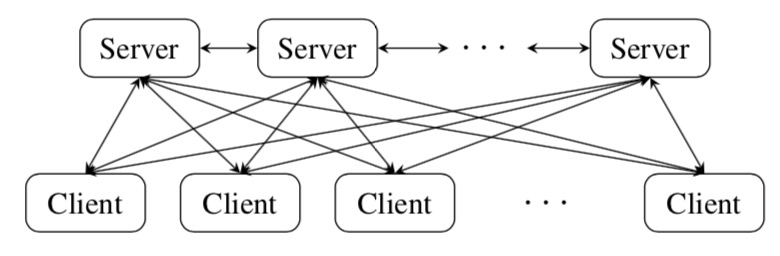
\includegraphics[width=10cm]{ps_comm_pattern}
\caption{参数服务器通信架构图}
\end{figure}
参数服务器主要有5大优点:(1)通信高效,在异步情况下不会拖慢计算;(2)支持弹性一致性,其可通过放宽模型一致性条件,达到算法收敛速度和系统性能之间的平衡。(3) 扩展性强,增加节点时无需重启网络;(4)机器错误恢复时间短,Vector Clock容许网络错误了;(5)易用性,其全局共享的参数使用向量和矩阵表示,而这些又可以用高性能多线程库进行优化。\\
参数服务器下,训练流程如图1.2所示。训练主要包含4部分:(1)worker节点各自计算梯度;(2)worker节点将各自梯度push到server端;(3)server端对所有梯度进行求和平均并更新模型参数w;(4)worker节点从server端pull最新的参数w。\\
\begin{figure}[htp]
\centering
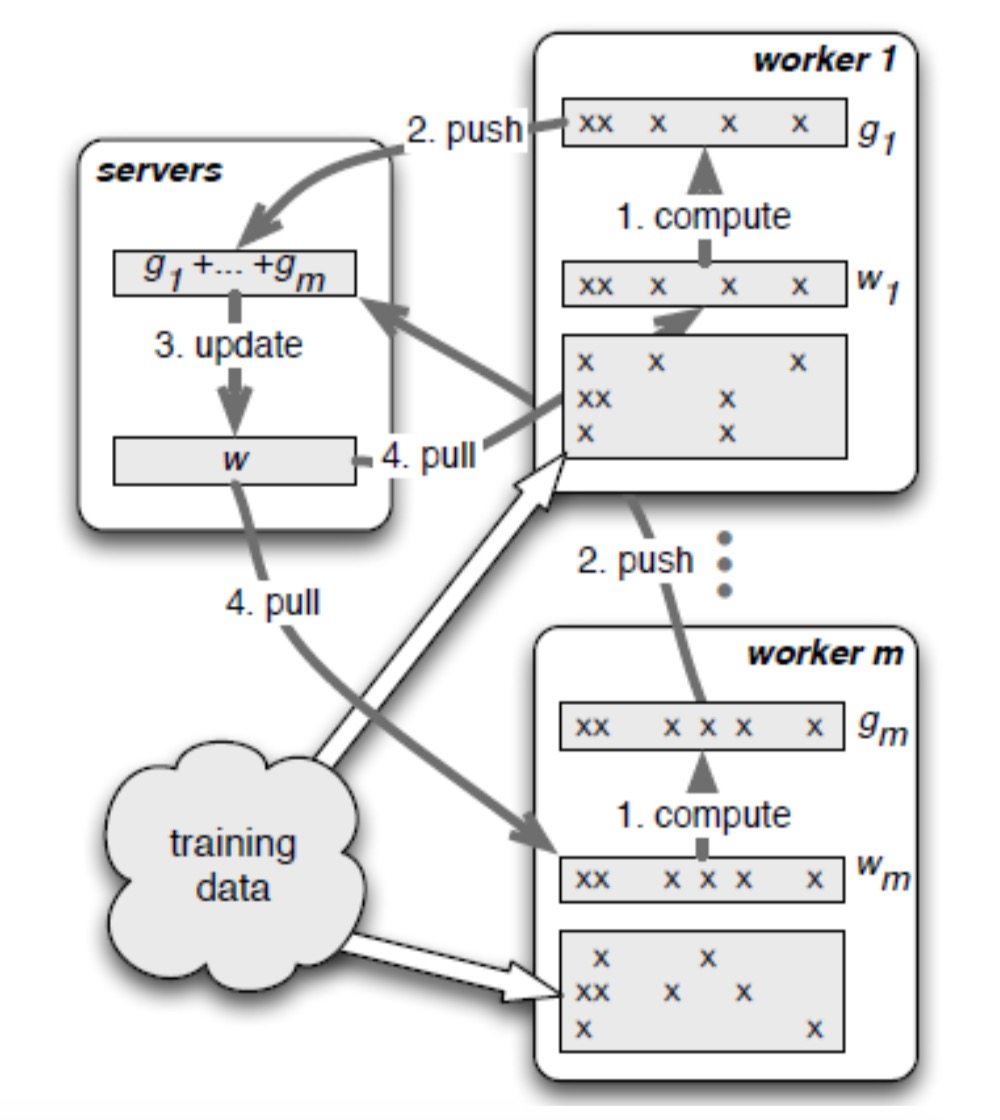
\includegraphics[width=10cm]{ps_update_way}
\caption{参数服务器下训练流程图}
\end{figure}
horovod\upcite{horovod2018}是uber基于百度ring-allredue的通信方式,提出了的分布式通信框架,因为其优异的性能和简单的使用方式,在业界引起广泛关注。horovod基于mpi实现,为提高分布式通信的效率,提出tensor fusion和分层级同步策略等方法,极大提高了分布式训练效率。

\subsection{目前业界最新训练硬件:fp16,bf16训练}
因为传统硬件计算基本以浮点数为主,目前绝大多数训练场景中都采用浮点数运算。而神经网络本身就存在随机性和容错性的特点,其计算精度并不需要达到浮点数的精度,为了节省内存,带宽,以及在支持低精度计算的硬件设备上提升计算效率,业界提出了两种主流的低精度数据格式用于训练神经网络。分别是IEEE半精度fp16和bfloat16格式。经过工业界验证,用这两种数据格式训练神经网络均保证训练精度,逐渐成为主流。\\
2017年Micikevicius P等为节省训练的内存开销,提出混合精度训练\upcite{mixed2018}的方法,使用IEEE半精度格式存储所有网络层的中间结果。相对于原始32位浮点数计算而言,训练网络模型所消耗的内存减小了一半;同时,为了弥补半精度表示所带来的损失,文章提出混合精度更新方法,如图1.3所示。在设计损失函数时,适当放大损失函数权重的方法来保证训练精度。\\
\begin{figure}[htp]
\centering
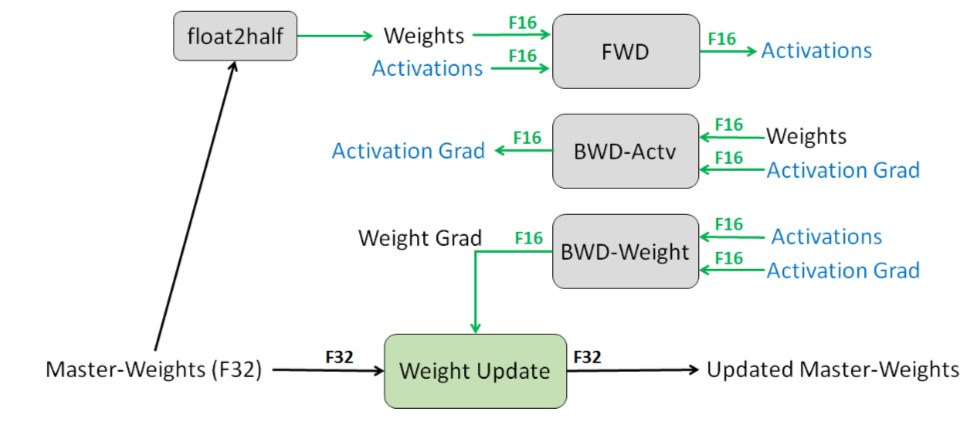
\includegraphics[width=10cm]{fp16_training_steps}
\caption{混合精度训练迭代方法}
\end{figure}
文章也指出,当前大部分硬件不支持半精度计算,所以此方法在现有硬件基础上只能节省内存,由于实际计算是先把半精度数值转换成浮点数再计算,存在一定的额外开销,使得计算速度相对有所下降。目前Nvidia的最新硬件,如Volta系列,turing系列已经支持半精度计算,可进一步提升计算效率。\\
目前,支持bfloat16计算的硬件只有google的TPU。受硬件限制,深度学习框架中只有tensorflow对bfloat16提供了数据支持,其他框架如pytorch,mxnet等则暂时不支持。

\section{本文工作}
本课题根据现有硬件特点,提出两种分布式数据同步方式,在保证训练精度的情况下,通过减小网络通信量,以减小通信开销,提高训练效率。第一种是半精度同步方式;第二种是bfloat16同步方式。因为目前以mpi为基础的horovod通信框架效率高于parameter servers,所以本文基于horovod实现这两种同步方式。下面对其主要实现过程以及需要利用的相关知识进行介绍。
\subsection{半精度同步方式}
根据现有硬件特点可知,现阶段绝大部分硬件只支持浮点运算,即使目前主流深度学习框架支持半精度训练,其做法只是将半精度输入转换成浮点数再进行计算,使得计算效率低于正常浮点计算。而根据神经网络的特点,半精度数据即可满足其训练需求。\\
分布式训练相对于单机训练方式而言,仅多了同步梯度的过程,其同步开销大小决定了分布式训练效率的高低。考虑到现有硬件的特点和深度学习对半精度数据的友好性,本文提出使用浮点数据计算,半精度梯度数据同步的训练方法。通过减少网络通信量的方法,提高分布式训练效率。本文提出的半精度同步方式,主要包含下面三步:\\
1. 在进行梯度同步之前,将各层梯度转换成半精度表示,对于超过半精度表示范围的梯度,通过阈值截取的方式将其转换成固定的大小,避免无效数据的产生;
2. 基于horovod实现自定义的半精度加法,在实现过程中为弥补数据转换导致的信息损失,将梯度转换为浮点数进行求和并适当增大梯度权重,将其传入mpi用于梯度求和;
3. 在完成半精度同步后,将半精度的梯度转换为浮点数表示,用于下一次迭代计算。

\subsection{bfloat16同步方式}
bfloat16数据格式所需的数据位与半精度数据格式一致。其传输的数据量不变,而其指数位与浮点数一致,精度位比浮点数少了16位。相对于半精度数据而言有两个优势:1.在与浮点数进行转换的过程中,直接将浮点数的低16位舍去即可,无需对数据位进行转化。其与浮点数的转化更为高效;2.因为其指数位长度与浮点数一致,故其表示范围与浮点数基本一致,在进行数据转化时,不存在数值越界的情况。同时,因为bfloat16指数位相对较长,使得其精度位相对较短,其表示的精度相对半精度数据要差。\\
bfloat16同步方式的实现方法与半精度数据同步方式相似,包含下面三个步骤:
1. 在进行梯度同步之前,将各层梯度转换成bfloat16数据格式;
2. 基于horovod实现自定义的bfloat16的加法,将其传入mpi用于bfloat16梯度的求和;
3. 在完成bfloat16数据同步后,将blfloat16的梯度转换为浮点数表示,用于下一次迭代计算。
\section{本文组织结构}
本文针对现有硬件特点和神经网络对低精度数据的友好性,提出两种低精度数据传输方式,在保证训练精度的前提下,减小数据通信量,提升了分布式训练效率。文章主要探讨了在分布式训练神经网络中低精度数据传输的可行性以及不同数据表示的优劣点。本文主要分为五章,详细安排如下:\\
第一章,绪论。主要对本课题的研究背景和研究意义进行介绍,系统介绍了目前以神经网络为主的深度学习的发展,分布式深度学习系统的发展和低精度训练神经网络的最新进展以及现阶段计算硬件的限制。并说明了本文的主要研究内容以及对应的创新点。最后说明了本文的组织结构。\\
第二章,分布式训练神经网络和低精度训练的相关研究。\\
第三章,。。。\\
第四章,。。。\\
第五章,。。。\\









\chapter{分布式深度学习相关研究}
本章主要介绍分布式深度学习系统涉及的相关技术。从分布式深度学习系统的特点出发,阐述其中设计的难点和重点。从精度和效率两方面分析分布式深度学习系统的特点,并介绍近年来神经网络在不同领域的发展以及目前业界对分布式深度学习的研究进展。
\section{分布式训练神经网络的特点}
随着网络模型的不断增大,数据日益增加以及应用需求的剧增,在深度学习发展历程中,分布式训练神经网络是必不可少的一环。目前主要有数据并行和模型并行两种方法用于分布式训练,如图\ref{fig:data_model_parallel}所示。

\begin{figure}[htp]
\centering
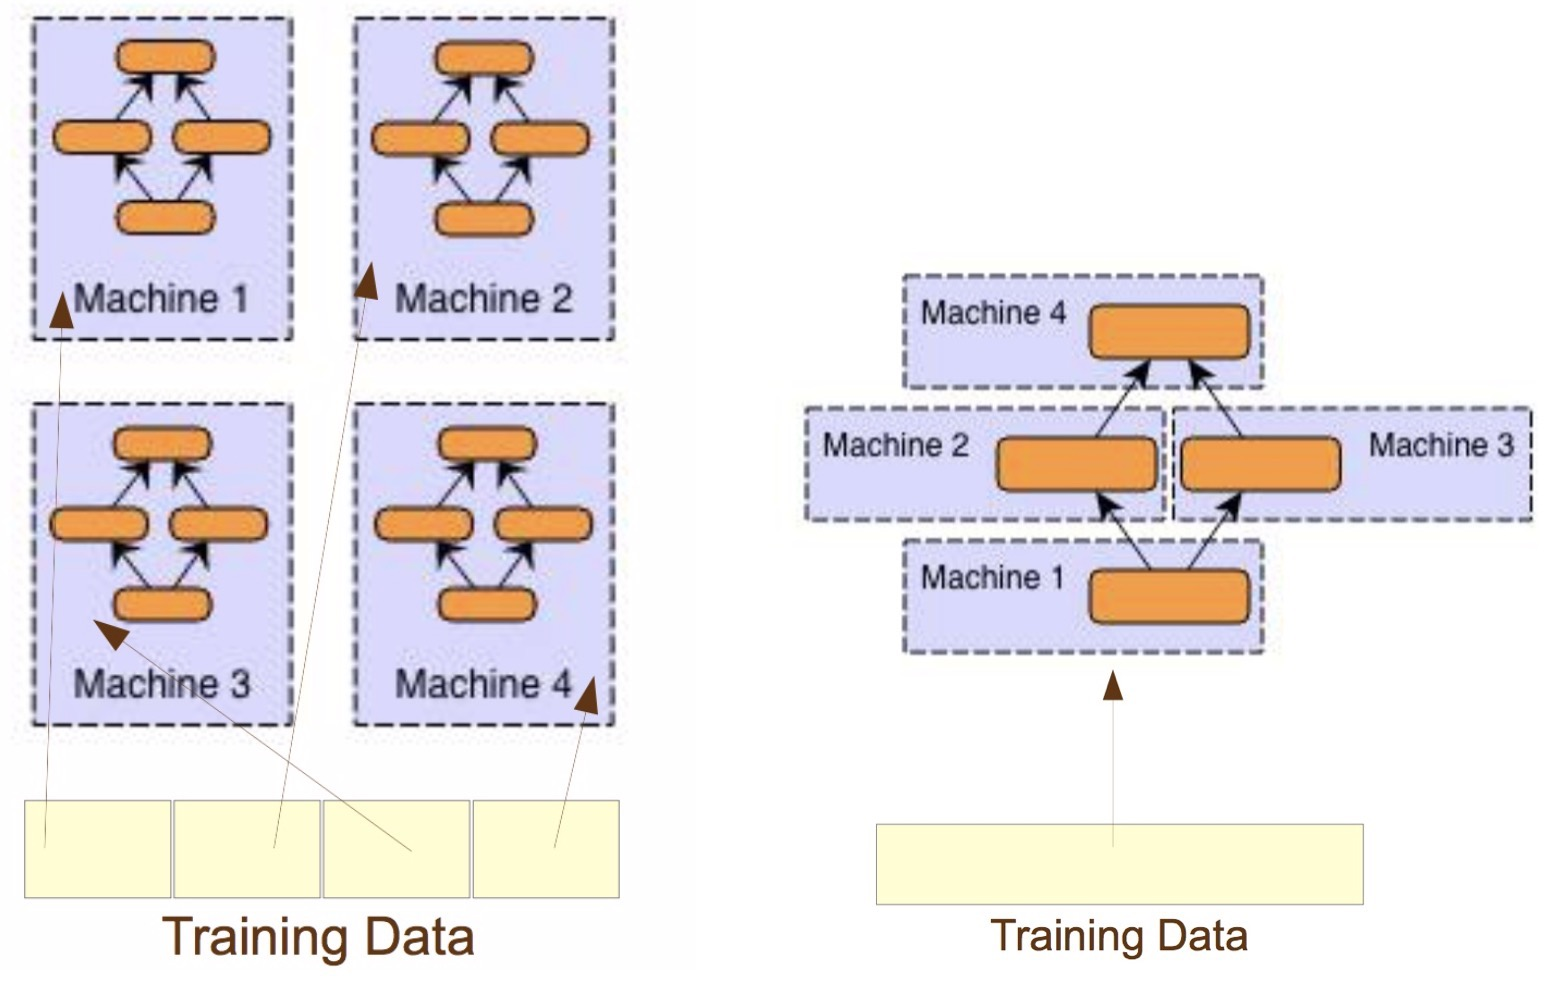
\includegraphics[width=13cm]{data_model_parallel}
\caption{数据并行(左)与模型并行(右)示意图}
\label{fig:data_model_parallel}
\end{figure}
数据并行是把数据分到不同的计算节点上,让不同节点处理不同的数据。因为有多个节点在并行地处理数据,所以在单位时间内,理应能够处理更多的数据,也即达到了并行计算的目的。模型并行则是把一个大的网络模型划分成很多小块,然后把每小块对应的参数、状态和计算任务分到不同的计算节点上执行,类似于流水线作业。模型并行除通过模型并行获得加速外,当某些模型在单机上无法训练的时候(如内存不够),则只能通过模型并行才能完成训练。目前业界绝大部分训练以数据并行的方式进行训练。

分布式训练神经网络主要有两个指标:一是精度,即随着分布式规模不断增大,在数据并行方法下必然导致用于训练的神经网络的batch size线性增大,即每次迭代更新所用的数据增多,而整体的迭代次数线性降低。当batch size增长到接近数据集大小时,sgd算法就不再适用。在大batch size情况下,如何保证单机batch size一样的精度是分布式深度学习中重要难题。尤其是在分布式规模较大情况下,传统sgd更新算法已经无法保证训练精度,需要新的更新算法保证网络精度。如facebook提出的热启动、线性增大学习率方法\upcite{train1hour2017},在保证训练精度情况下,将batch size提升至8k;伯克利的尤洋等\upcite{train24min2017}提出的分层自适应学习率的方法,进一步将batch size提升至32k;以及谷歌大脑\upcite{dontdecay2018}提出通过逐渐增大batch size替换学习率衰减的方法,最终将batch size提升至64k,只用两千五百多次迭代将ImageNet训到了理想精度。二是效率,即在保证精度的情况下,训练系统的效率要尽可能高,分布式相对于单节点的加速比越接近理想加速比则系统可扩展性越好。而根据分布式训练更新特点可知,分布式训练相对于单机训练区别在于多了同步全局梯度的开销,计算开销与单机相同。故同步梯度开销的大小对分布式深度学习系统的训练效率和可扩展性好坏至关重要。

为减少同步梯度的开销,涌现出了一系列异步,半异步的方法,如Hogwild\upcite{hogwild2011}提出lock free方法,在稀疏问题上具有显著效果;Sixin Zhang等人提出弹性均值随机梯度下降算法\upcite{easgd2015},通过预估节点梯度与全局梯度的差值来弥补异步更新的不足,达到理想效果;Peter等\upcite{scaledist2016}提出gossiping sgd算法,类似于去中心化的EASGD算法,在节点规模较小的情况下,收敛速度快于传统sgd算法;随后,Ioannis Mitliagkas等\upcite{asynmomentum2016}提出一种新颖的momentum更新方法,将节点梯度与全局梯度的差距当成隐含的momentum来解释,从而提出通过设置反向momentum的方法抵消局部梯度与全局梯度之间的差异。

目前神经网络的训练基本是用sgd算法或sgd算法的变种。在分布式训练神经网络中,异步或半异步的sgd算法无法达到正常收敛水平,能够保证神经网络收敛精度的异步或半异步的更新算法有待科学家进一步研究探索。目前分布式训练神经网络主要采用严格同步的更新方法,这使得提高训练系统效率更为困难。
\section{神经网络的发展}
近年来神经网络因其突出的性能在各个领域得到广泛应用。下面分别从图像分类、物体检测、自然语言处理三个领域对神经网络发展的进行介绍。
\subsection{神经网络在图像分类领域的发展}
AlexNet\upcite{alexnet2012},将卷积神经网络用于图像分类的开山之作。2012年在ImageNet上刷新各项纪录,夺得冠军,掀起一股神经网络热潮。其网络结构如图~\ref{fig:AlexNet}所示。受当时设备算力和显存的影响,作者将模型放在两块GPU上共同训练,网络总共8层。最终以超过第二名8.2\%的分数夺得冠军。

\begin{figure}[htp]
\centering
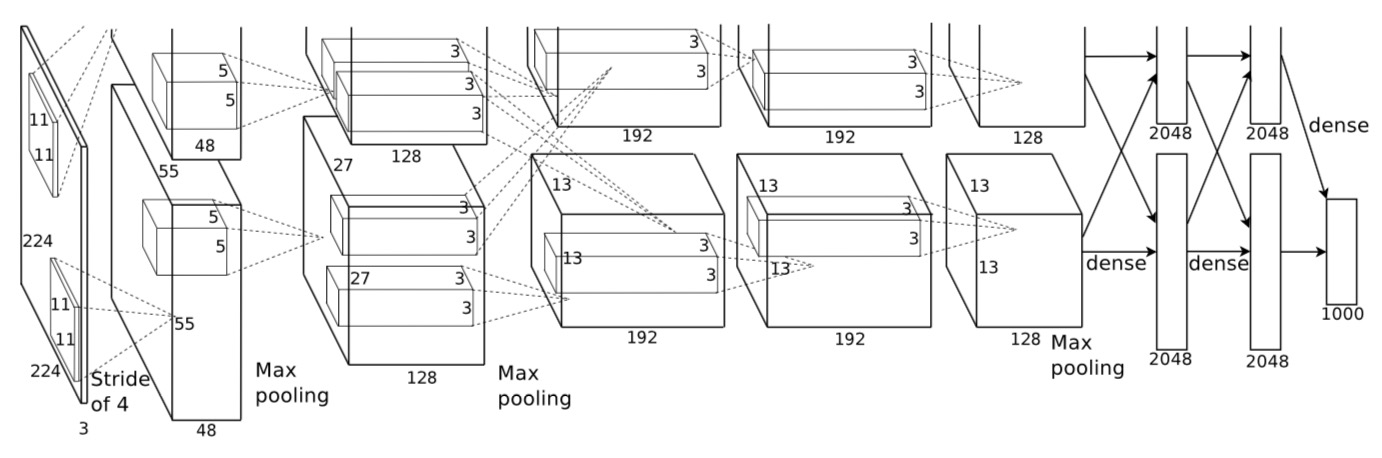
\includegraphics[width=13cm]{AlexNet}
\caption{AlexNet网络结构示意图}
\label{fig:AlexNet}
\end{figure}
随后,DeepMind提出了性能更强网络结构更深的VGG\upcite{vgg2014}系列网络。同时相对于AlexNet,该网络结构也更加规则化,为神经网络提供了一个模块化设计的思路,为以后设计更大更深的网络提供思路。此后基于卷积神经网络的各种基本组件,就可以像搭积木一样设计出相应的网络结构。

同时,google也提出性能更强,类似网中网的网络结构Inception\upcite{inception2015}系列。即网络的基本组件不再是简单的单层结构。而是偏复杂的module结构,类似一个小型的网络模块,如图~\ref{fig:inception_picture}所示。

\begin{figure}[htp]
\centering
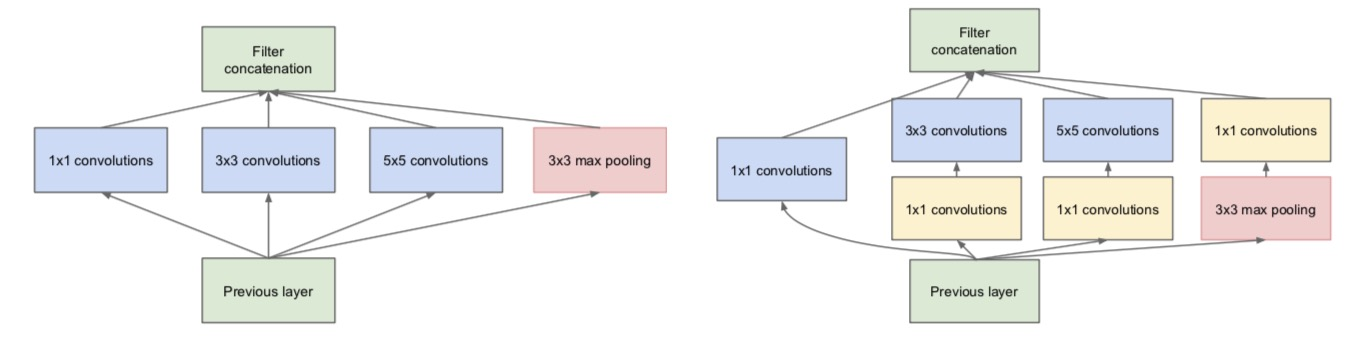
\includegraphics[width=12cm]{inception_picture}
\caption{inception module结构示意图}
\label{fig:inception_picture}
\end{figure}
如图~\ref{fig:inception_picture}分别展示了下采样和不下采样情况下,module的结构模型。随后基于inception提出了一系列的改进版如inception-V2,inception-V4等。从中可以看出网络设计越来越趋向于结构化。卷积核的形状也越来越规整,基本以3x3卷积为主,没有了诸多不同尺寸的卷积核设计。

随后,Kaiming He等\upcite{resnet2016}提出声名大噪的ResNet,一举夺得CVPR 2016年最佳学术论文奖。其计算量、参数量远小于VGG,inception,而精度则比其他网络要高。其核心思想来源于传统机器学习中的残差学习。提出让逐层网络学习上一层网络的残差,比直接学习特征要相对容易。基本残差结构如图~\ref{fig:resnet_block}所示。

\begin{figure}[htp]
\centering
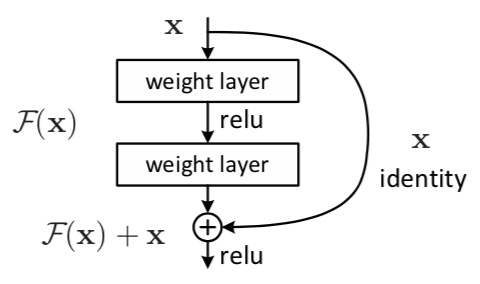
\includegraphics[width=10cm]{resnet_block}
\caption{ResNet block结构示意图}
\label{fig:resnet_block}
\end{figure}
2017年,Gao Huang等\upcite{denselynet2017}基于残差连接的思想,提出DenseNet。其核心思想是为了使后层网络获取前部分网络尽可能多的信息。使其分别与前面各层建立连接,从而形成相对密集连接的DensetNet网络,如图~\ref{fig:DenseNet_picture}所示。

\begin{figure}[htp]
\centering
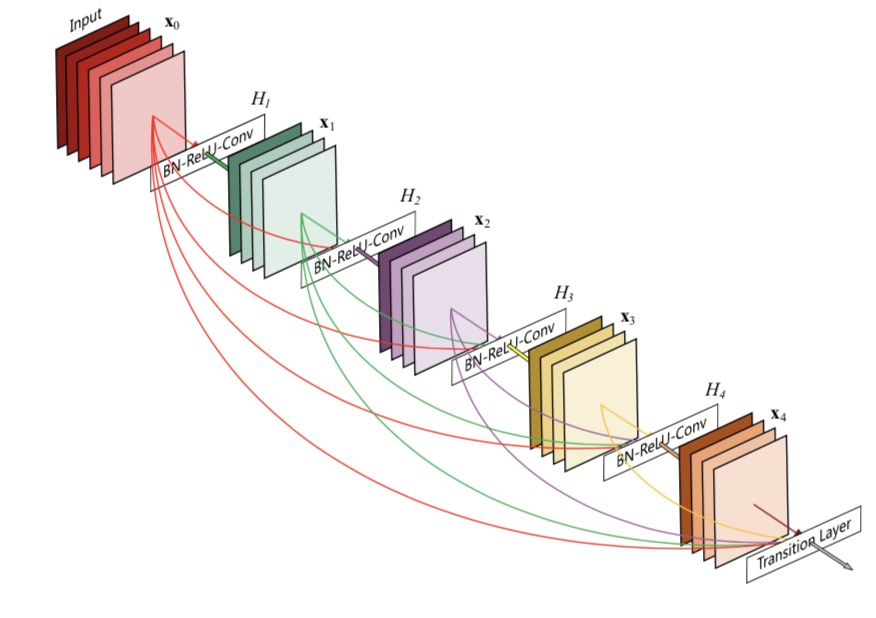
\includegraphics[width=12cm]{DenseNet_picture}
\caption{DenseNet结构示意图}
\label{fig:DenseNet_picture}
\end{figure}
随着越来越多的神经网络部署到实际应用中,其对网络计算量提出了许多限制要求。因为在算力受限的设备中如:手机,个人电脑以及其他嵌入式设备等,无法对计算量大的网络完成计算,或计算量过大则无法满足其实时性要求。受限算力下的小型网络结构应运而生。

2017年,Andrew G. Howard等\upcite{mobilenet2017}提出轻量级网络MobileNet。其核心思想是根据传统卷积的作用:扩大感受野和融合通道间的特征。分别用计算量偏小的depthwise convolution和pointwise convolution代替,极大减少了网络的计算量,其替换原理图如图~\ref{fig:mobilenet}所示。在相同计算量的情况下,达到了非常好的性能。

\begin{figure}[htp]
\centering
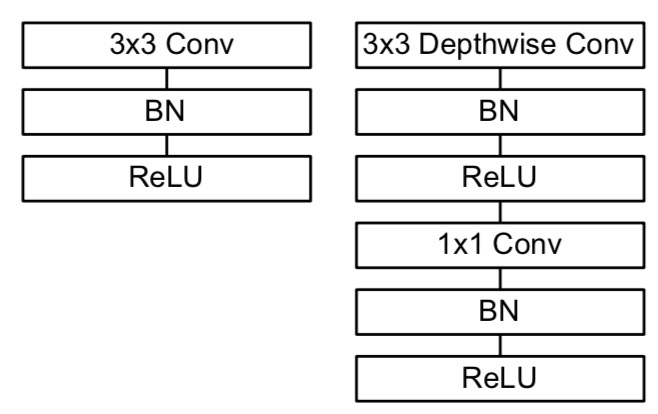
\includegraphics[width=12cm]{mobilenet}
\caption{传统conv+BN+Relu(左)与depthwise separable conv(右)示意图}
\label{fig:mobilenet}
\end{figure}
随后,Xiangyu Zhang等\upcite{shufflenet2018}提出ShuffleNet,进一步减小了网络计算量。在相同计算量情况下,网络性能达到最好情况。其核心思想是把pointwise convolution进行分组,根据卷积计算公式可知,分组越多,计算量越少,通道间信息传递也越少。为了使通道间信息能更好的融合,论文提出shuffle的方式将各层通道的信息进行融合,示意图如图~\ref{fig:shufflenet}所示。其主要包含两个步骤:一是对pointwise做分组卷积;二是对分组后的卷积在通道之间做shuffle,以保证通道间的信息融合。

\begin{figure}[htp]
\centering
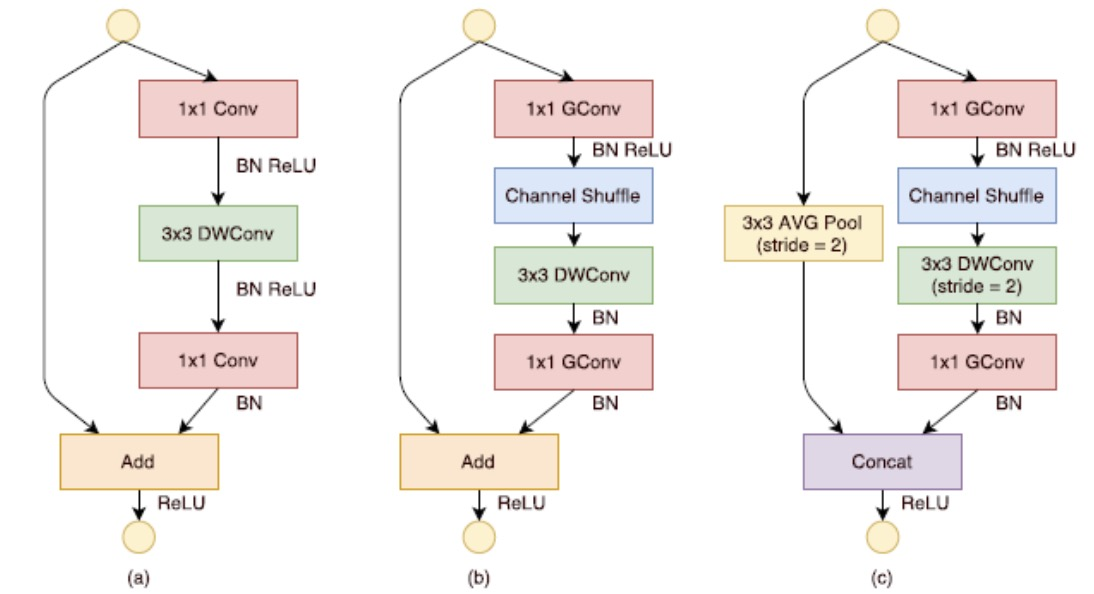
\includegraphics[width=14cm]{shufflenet}
\caption{bottleneck单元(a)组卷积单元(b)stride=2的组卷积单元(c)示意图}
\label{fig:shufflenet}
\end{figure}
\subsection{神经网络在物体检测领域的发展}
随着神经网络在图像分类领域取得的显著进展,人们开始将卷积神经网络应用于物体检测领域。近年来卷积神经网络在该领域也取得了突飞猛进的发展。目前基于神经网络的检测算法主要分为两种:一阶段检测网络和二阶段检测网络。一阶段网络速度较快,精度偏低;二阶段网络速度偏慢,精度较高。下面分别介绍一阶段网络和二阶段网络中相关的研究进展。

2014年,Ross Girshick等\upcite{rcnn2014}提出的R-CNN网络是将神经网络用于目标检测领域的开山之作。其主要分为三个步骤:1.用传统方法selective-search从原始图片中选取出2k个框;2. 将这些框对应的图片送入卷积神经网络,提取对应框的特征;3.使用传统SVM分类器对得到的特征进行分类。其算法流程图如图~\ref{fig:rcnn_overview}所示。

\begin{figure}[htp]
\centering
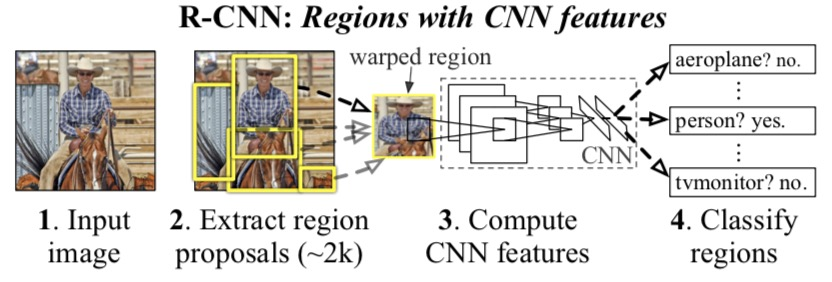
\includegraphics[width=12cm]{rcnn_overview}
\caption{R-CNN算法流程图}
\label{fig:rcnn_overview}
\end{figure}
由其算法流程图可知,该算法流程耗时较复杂。因为一张图片同时提取2k个框,提取的特征数据量巨大,占用磁盘空间较大,如5000张图片会产生几百G的特征文件,且因为一张图片中的每个特征框都得过一遍神经网络,其处理速度非常慢,平均47秒处理一张图片。

针对R-CNN训练速度慢的问题,2015年Kaiming He等\upcite{sppnet2014}提出SPPNet。其分析了R-CNN之所以速度慢的原因在于一张图片要过2k次神经网络。根本原因在于不同框的尺寸不同,而网络最后的分类部分要求特征图尺寸一致,这种矛盾使得2k个框只能分别输入神经网络。为克服这个问题,论文提出空间金字塔池化方法,其结构示意如图~\ref{fig:sppnet}所示。通过该方法将不同尺寸的特征图池化到相同尺寸,从而使得一张图片只需过一遍神经网络,极大提升了网络性能。

\begin{figure}[htp]
\centering
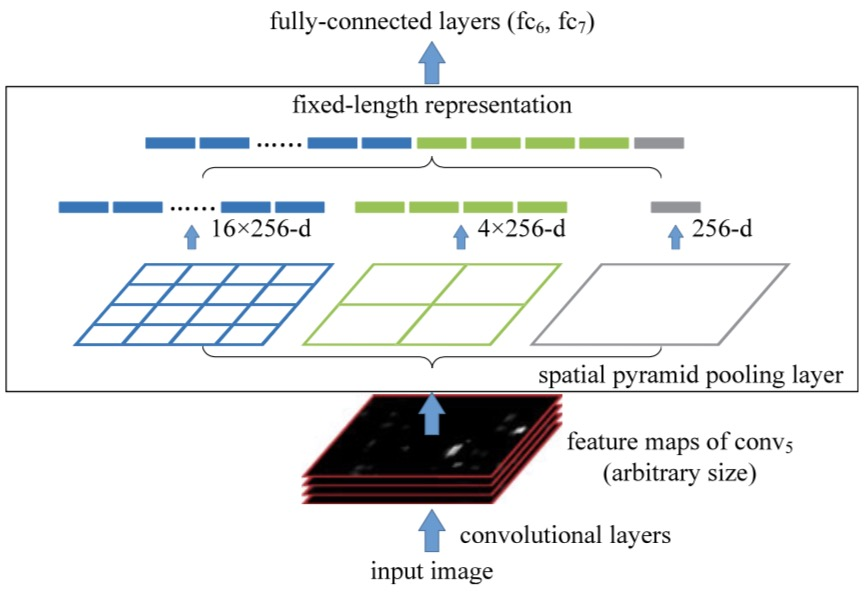
\includegraphics[width=10cm]{sppnet}
\caption{SPP结构示意图}
\label{fig:sppnet}
\end{figure}
随后,Ross Girshick根据R-CNN的缺点,以及SPPNet的优点,提出Fast R-CNN\upcite{fastrcnn2015},主要有两个工作:1.将R-CNN中SVM的分类部分用卷积神经网络代替;2.改进SPP的池化方法,提出ROI pooling方法。Fast R-CNN的网络结构如图~\ref{fig:fast_rcnn}所示。

\begin{figure}[htp]
\centering
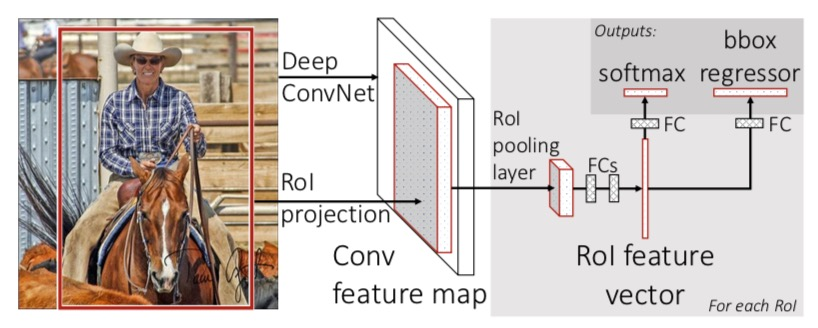
\includegraphics[width=10cm]{fast_rcnn}
\caption{Fast R-CNN算法流程图}
\label{fig:fast_rcnn}
\end{figure}
基于Fast R-CNN的工作,Shaoqing Ren, Kaiming He和Ross Girshick进一步提出Faster R-CNN\upcite{fasterrcnn2015}检测网络。为了解决Fast R-CNN网络提取框耗时的问题,论文提出用于提取检测框的FPN网络,进一步提升了训练速度,实现了真正意义上的端到端训练。FPN网络结构如图~\ref{fig:fpn}所示。随后也出现了各种网络如:R-FCN\upcite{rfcn2016},focal loss\upcite{focalloss2017}等。

\begin{figure}[htp]
\centering
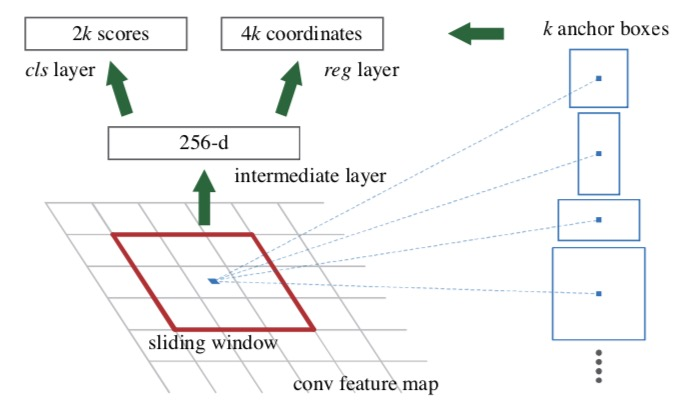
\includegraphics[width=10cm]{fpn}
\caption{FPN网络结构图}
\label{fig:fpn}
\end{figure}
另一方面,一阶段目标检测网络也发展迅猛。2016年,Joseph Redmon等提出yolo网络\upcite{yolo2016},其核心思想是直接让网络预测出每个特征点的类别和对应框的4个坐标。其网络结构如图~\ref{fig:yolo}所示。因其检测速度快的优势,得到广泛使用,随后基于yolo不断进行改进,yolo2,yolo3也相继发表提出。

\begin{figure}[htp]
\centering
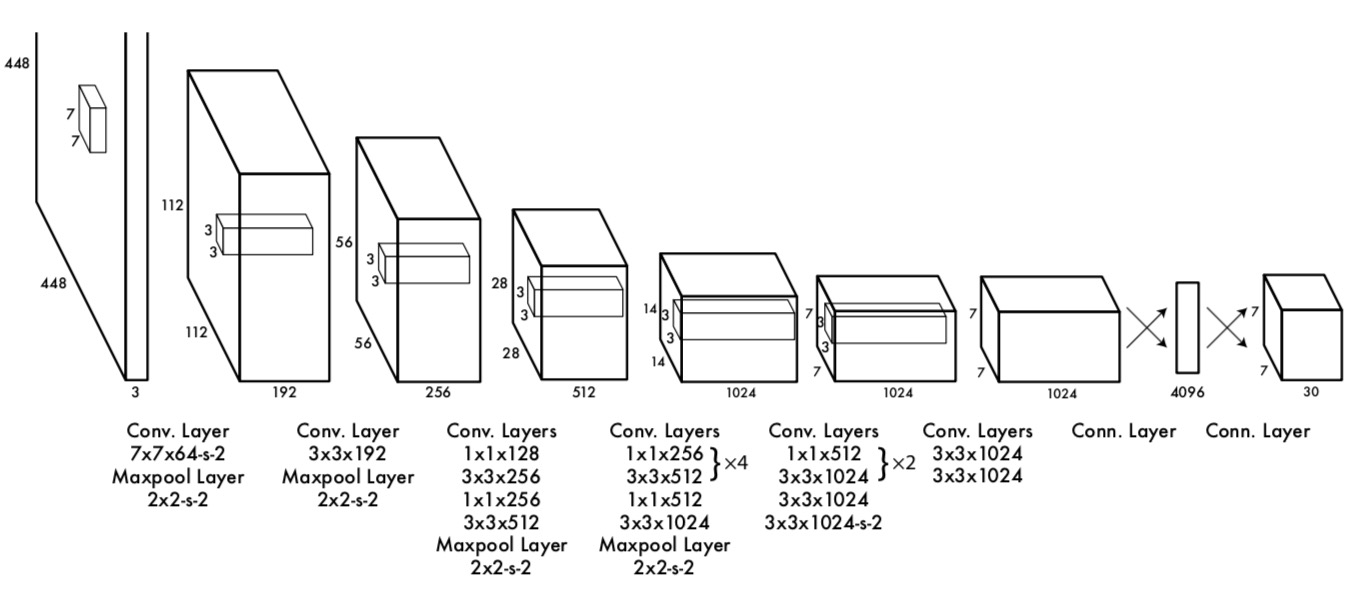
\includegraphics[width=14cm]{yolo}
\caption{yolo网络结构图}
\label{fig:yolo}
\end{figure}
同年Wei Liu等提出SSD网络\upcite{ssd2016},结合了Faster R-CNN和yolo的优点,采用了Faster R-CNN的anchors机制,同时是和yolo相同的一阶段检测方法。网络结构如图~\ref{fig:ssd}所示。其使用不同层的feature map预测不同的大小的框,不同层的feature map可以预测不同大小的物体,达到预测不同大小物体的目的。

\begin{figure}[htp]
\centering
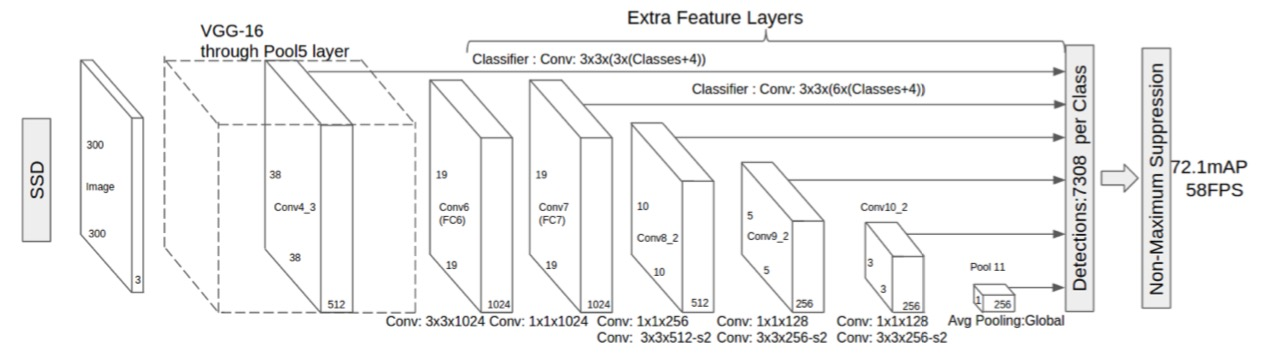
\includegraphics[width=14cm]{ssd}
\caption{ssd网络结构图}
\label{fig:ssd}
\end{figure}
\subsection{神经网络在自然语言处理领域的发展}
在自然语言处理领域,神经网络被用在了机器翻译,文本处理,阅读理解等诸多方面。2016年,谷歌提出其机器翻译模型GNTMT\upcite{gnmt2016}。其引入了注意力机制使得系统处理长句子时更准确高效。针对神经网络系统的三个弱点:1.训练速度很慢并且需要巨大的计算资源。由于参数量计算量过大,其翻译速度也远低于传统的基于短语的翻译系统;2.对罕见词的处理很无力,传统神经网络直接复制原词的方式在很多情况下不是一个好的解决方法;3.在处理长句子的时候会有漏翻译的现象。GNMT使用了8层含有残差连接的循环神经网络,其结构如图~\ref{fig:gnmt}所示。残差连接可以帮助某些信息的传递,比如梯度、位置信息。同时,attention层与decoder的底层以及encoder的顶层相连接。

\begin{figure}[htp]
\centering
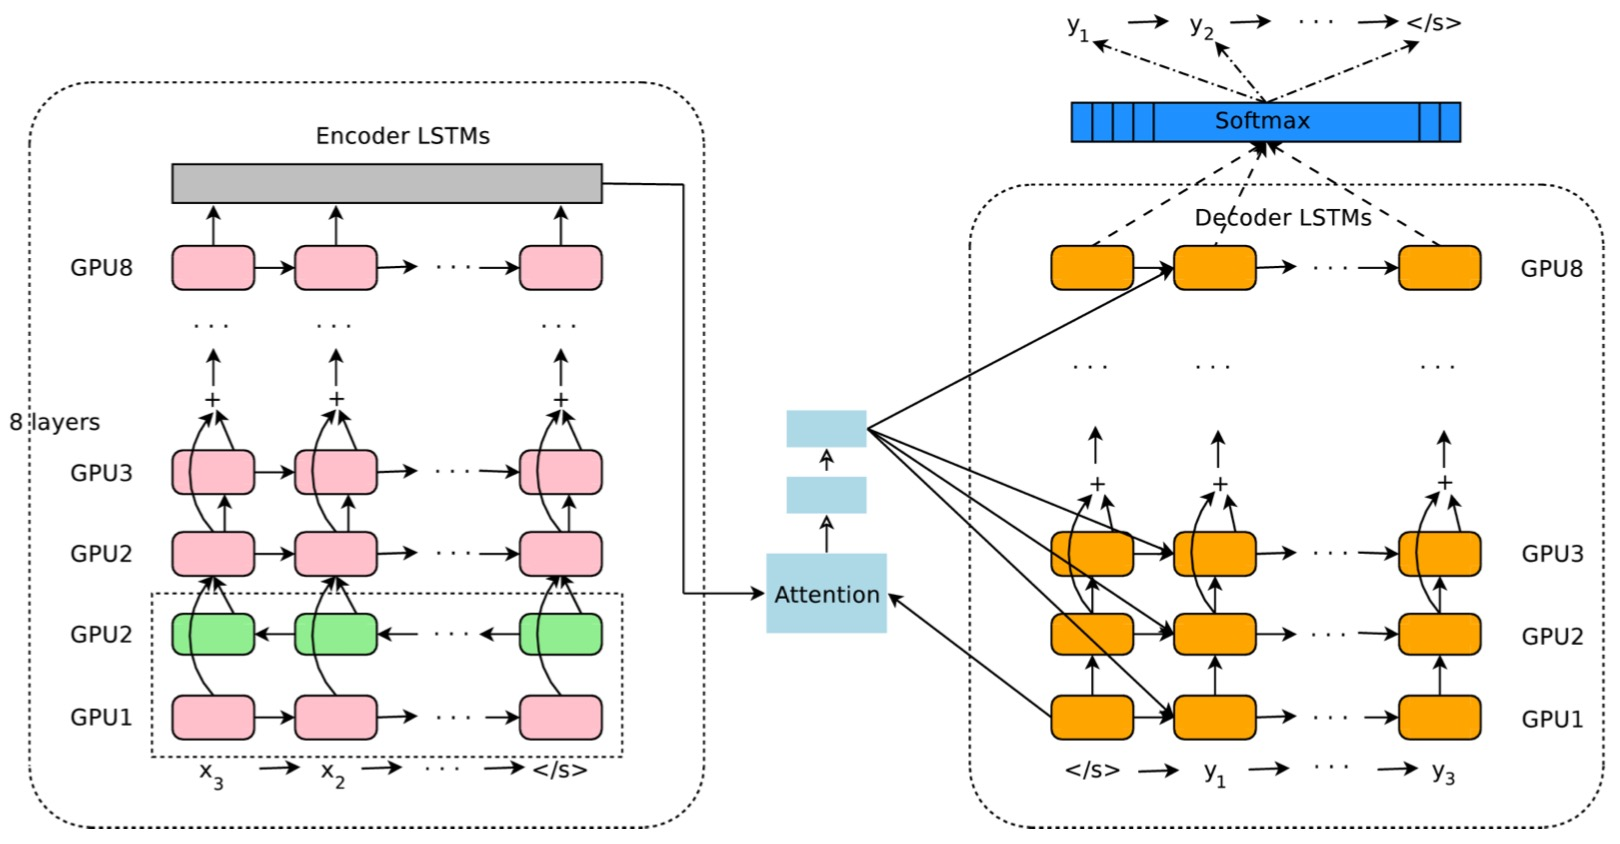
\includegraphics[width=14cm]{gnmt}
\caption{gnmt网络结构图}
\label{fig:gnmt}
\end{figure}
2018年,谷歌提出BERT\upcite{bert2018}模型,刷新了多项NLP任务的成绩,是一项里程碑式的工作。使用了masked lm和下一句预测的联合训练方法,在加上12层的transformer。
\section{分布式深度学习的发展}
分布式深度学习涉及到的领域很广。涵盖优化算法、模型、系统和应用等。下面分别介绍以下三个方向的研究进展:分布式系统、优化算法和数据压缩。
\subsection{分布式深度学习系统的发展}
自2012年底AlexNet\upcite{alexnet2012}在ImageNet上大放异彩,刷新诸多记录,从此开启了深度学习的新篇章。同年,对应的分布式深度学习系统也应运而生。Jeffrey Dean等提出的DistBelief\upcite{distbelief2012},即Google的第一代深度学习系统,其核心实现是把分布式机器学习里面的数据并行(data parallelism)和模型并行(model parallelism)用在深度学习上,通过这两种并行方法把深度学习大规模部署到集群。同时,论文提出了分布式异步SGD—DownPour SGD和L-BFGS算法,在CPU集群上系统效果显著。

随后,考虑到分布式训练网络过程中的同步通信开销,Qirong Ho等\upcite{ssp2013}提出了松弛一致性模型:Stale Synchronous Parallel(SSP), 如图~\ref{fig:ssp_picture}所示。解决了严格同步(BSP)模型下木桶效应导致同步时间过长的问题,提高了计算效率。并基于该模型,搭建了Petuum系统。

\begin{figure}[htp]
\centering
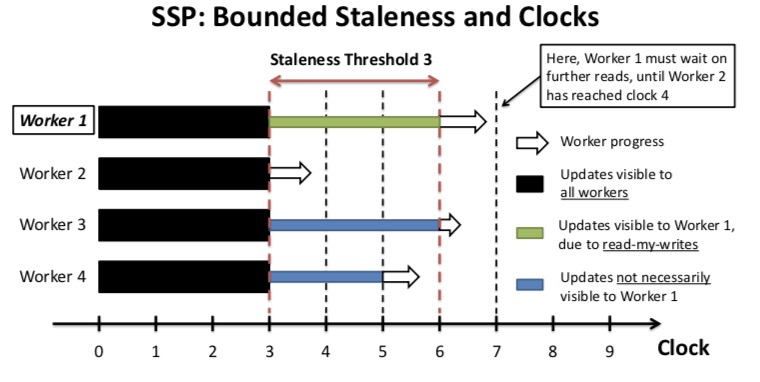
\includegraphics[width=12cm]{ssp_picture}
\caption{SSP模型示意图}
\label{fig:ssp_picture}
\end{figure}
同时期,Adam Coates等\upcite{cots2013}搭建了一个GPU集群:COTS HPC system,该系统通过模型并行方法分布式训练网络模型。因为该系统使用GPU计算,CPU用于通信。在InfiniBand 50 Gb网络上测试,计算在毫秒级完成,而通信时间则需要8秒,系统效率极差,为克服通信瓶颈,其提出一种复杂有效的GPU协作算法,进一步了提升集群效率。

紧接着Microsoft推出了基于参数服务器的深度学习系统Adam\upcite{adam2014}。其是一个CPU集群,通过模型并行的方式训练神经网络。为避免数据处理速度跟不上,系统专门用四台机器用于数据预处理,并将模型放在L3 cache上。为了提升网络间数据的传输性能,该系统设计了一种专门的网络IO,避免不必要的数据拷贝、传输。

分布式深度学习中一个关键的通信组件是参数服务器(Parameter Server),最早由Alex Smola提出,因其简单、高效的特点,被广泛用于分布式深度学习进行参数同步。最著名的参数服务器框架要数李沐等人做的Parameter Servers\upcite{ps2014},并进一步开发出MXNet。在李沐等人的Parameter Servers框架中,其集成了传统分布式框架Hadoop、Spark的优点,通过图遍历、消息压缩和去中心化等优化方法,理论性能与allreduce一致,实际性能十分优异,但其对CPU需求较大,当CPU承担任务过多时,容易因为竞争冲突导致性能下降。

随后,Henggang Cui等\upcite{geeps2016}在GPU上实现了Parameter Servers,推出GeePS系统,避免了CPU通信过程中GPU与CPU之间的数据拷贝,提高了数据通信效率。同时为缓解模型占用GPU显存过多的问题,提出一种GPU内存管理机制,使得在GPU受限情况下,训练更大的网络成为可能。
\subsection{分布式深度学习中优化算法的发展}
在分布式深度学习系统中主要分为异步算法和同步算法。下面分别介绍分布式深度学习中近年来异步和同步算法的研究进展。

2011年,Feng Niu等\upcite{hogwild2011}针对稀疏求解问题,提出异步更新方法即lock-free方法。因为是稀疏问题,每个worker需要更新的参数几乎均不一样,重叠率很低。所以不用以严格顺序更新,异步更新即可。2014年,Henggang Cui等\upcite{absp2014}提出一种结合ssp和wpc-bsp的算法A-BSP。算法原理图如图~\ref{fig:a_bsp}所示。大致内容为:在bsp中每次迭代都同步更新梯度,使得同步等待的时间在总体训练时间过长。为了减少同步等待的时间比重,提出每间隔wpc次迭代才同步更新一次,减少同步等待时间占整体时间的比重。该算法每隔n个iteration才同步更新一次,等效于增大batch size。但与之不同的是在n个iteration之间各个worker会根据本地的参数更新。

\begin{figure}[htp]
\centering
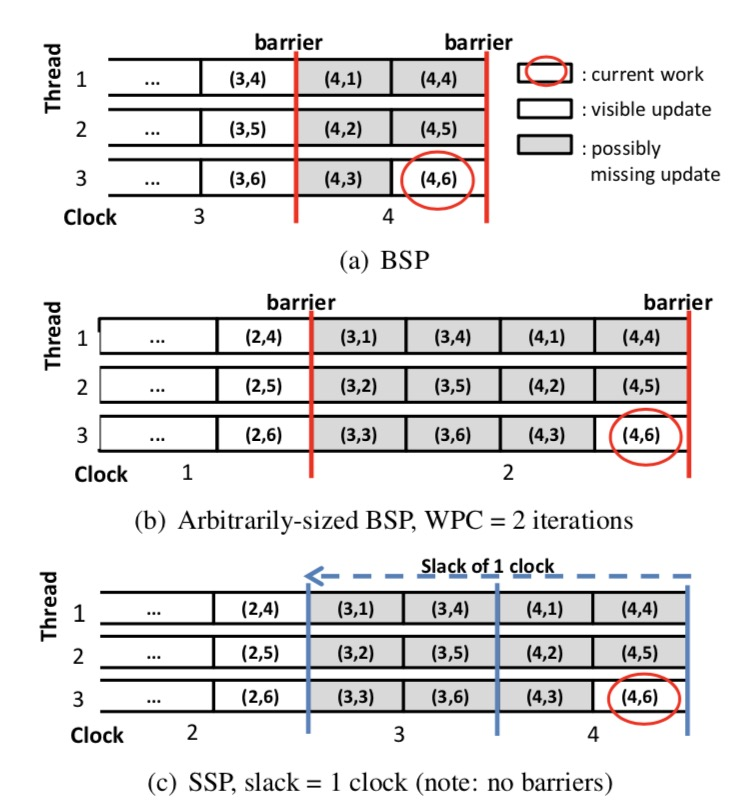
\includegraphics[width=12cm]{a_bsp}
\caption{bsp,a-bsp,ssp示意图}
\label{fig:a_bsp}
\end{figure}
2015年,Sixin Zhang等\upcite{easgd2015}提出异步的弹性均值sgd算法。其设计思想为:每个worker进行参数更新时,除了要考虑当前梯度,还应考虑当前worker的参数与中心节点master的全局参数的差距。不仅要减去当前worker的梯度,还应该减去这个差值。

随后,2016年Peter H等基于EASGD算法提出gossiping算法\upcite{scaledist2016}。与EASGD算法相似,是一个去中心化的EASGD算法,其将中心节点更新的全局参数直接用各worker参数的均值代替了。该论文实验结果有诸多启发性的结论:1. 在小节点情况下(节点数在32个以内),异步的EASGD,gossiping SGD收敛速度要快于同步SGD;2. 当节点数增大(到100节点),同步SGD的可扩展性更好;3. 当更新步长(即lr)较小时,同步SGD的收敛效果要好,即异步更新下,步长不宜太小;4. gossiping SGD单次迭代时间小于同步SGD,在训练刚开始阶段收敛速度很快,但当步长逐渐变小时,gossiping SGD的收敛速度变得很慢。

同时,Ioannis Mitliagkas等\upcite{asynmomentum2016}也在2016年提出一种通过调整momentum的值抵消异步更新梯度与全局实际梯度的差距。其设计思想是在异步SGD的情况下,每个worker求得的梯度并不是当前系统中最新权重的梯度,是相对较老权重的梯度,最新的权重梯度和计算出较老权重的梯度之间的差距实际上是一种隐含的动量。所以当使用异步SGD时,可以适当减小优化器中的momentum,因为异步SGD情况下本身就带有部分momentum,异步程度越大,即worker节点数越多,这种隐含的momentum就越大,此时优化器的momentum就应该越小。甚至优化器的momentum可以为负数,来抵消隐含momentum过大的影响。

该论文对异步更新方法提供了一种比较新奇的理解方式,但实际上关注点和EASGD,gossiping SGD是一致的,都是关注较老的参数与最新参数之间的差值。只不过EASGD,gossiping SGD是在worker的参数时,除了减去梯度,还减去了较老的参数与最新参数的差值。而本文虽然仅仅减去梯度,但通过调整momentum来弥补该梯度的不准确性。

由于在大部分神经网络中异步更新算法无法满足程序精度要求,实际应用中往往使用严格同步的更新算法保证训练精度。下面是同步更新算法的相关研究进展。

2017年,Hao Zhang等\upcite{posiedon2017}结合深度学习训练特点,针对严格同步优化算法进行了系统优化,极大提高了分布式训练效率。论文提出两个解决分布式训练中网络传输瓶颈的方法:1. wait-free backpropagation(WFBP),将反向传播和参数同步嵌套在一起,将大部分网络通信开销隐藏在反向求导的计算中,从而极大减小同步时间;2. SFB方法:在参数量很大的网络中,某些全连接层的参数量很大,会造成网络瓶颈,为了减少这部分网络传输参数,提出将全连接层的梯度(M*N)进行矩阵分解,得到(M+N)个参数,进行广播传输,然后再通过矩阵乘法将(M+N)个参数恢复成(M*N)的参数。通过上面两种优化方法,使得系统近乎达到理想的线性加速比,相对于原生框架的分布式效率有极大提升,如图~\ref{fig:poseidon_result}所示。

\begin{figure}[htp]
\centering
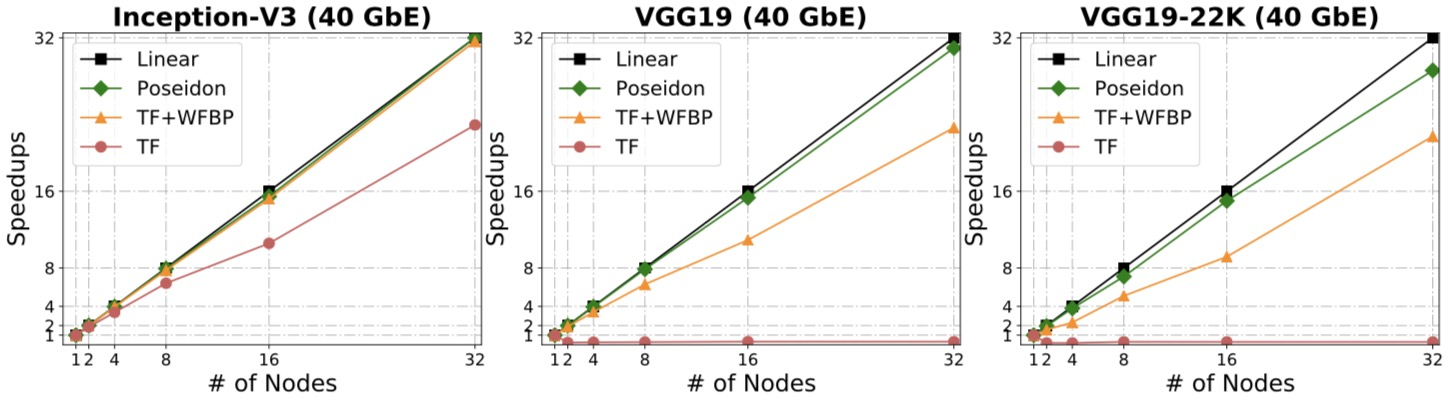
\includegraphics[width=14cm]{poseidon_result}
\caption{Poseidon实验对比图}
\label{fig:poseidon_result}
\end{figure}
由图~\ref{fig:poseidon_result}对比TF与TF+WFBP可知,WFBP算法对性能提升有巨大帮助,在参数量相对较小的网络(如inception-V3)中该算法即可保证网络达到近线性加速比。而在网络参数量较大,特别是全连接层参数量较大时,单使用WFBP算法不足以压缩同步参数的时间开销。因为全连接层计算量小而参数量大,使其对无法通过WFBP算法将通信延时隐藏在全连接层的反向计算中。而SFB算法正好解决了该问题。通过将全连接层M*N个参数分解成M+N个参数,极大减少了参数传输量。所以在全连接层占比较大的网络中,如VGG19,VGG19-22k等,加上SFB算法后分布式效率能接近理想加速比。

同年,Jianmin Chen等\upcite{bucketsgd2017}提出通过提供少量计算节点备份以缓解严格同步形成的木桶效应。论文首先通过大量实验验证了异步算法在神经网络训练中不能保证模型精度的问题,所以为保证训练精度应使用严格同步的优化算法。但是严格同步则导致每次迭代时间受计算最慢的机器的影响,随着集群增大,影响会越来越明显,为了避免这个影响,论文提出使用少量备份节点来减缓最慢机器导致的影响。假设集群中有53个计算节点同时计算,当server端接收到50个梯度后,就同步更新,剩下最慢的3个终止该次计算,这样能有效减少最慢的时间等待。这种通过备份节点来缓解木桶效应带来的影响具有非常好的启发意义。同时论文也提出下一步工作:用time-out,代替backup节点的想法要跟进。当80\%的梯度到达时,就更新参数,以这80\%的梯度代替所有的梯度进行更新。

同时,facebook等\upcite{train1hour2017}在Training ImageNet in 1 hour中提出两个简单且极为有效的调整学习率的方法:线性增大学习率和热启动方法。首先论文从sgd算法意义出发,从公式中推导出:当增大batch size时,线性增大学习率情况下,公式与原始batch size下的含义相同。同时在实际训练过程中,因为刚开始网络状态受初始化影响较大,且训练初期网络状态波动很大。学习率过大时,容易造成网络不收敛,故在训练刚开始阶段提出使用热启动的训练方法,从一个较小的学习率逐渐增长至线性增大策略所要求的学习率。实验结果如图~\ref{fig:training1hour_result}所示。

\begin{figure}[htp]
\centering
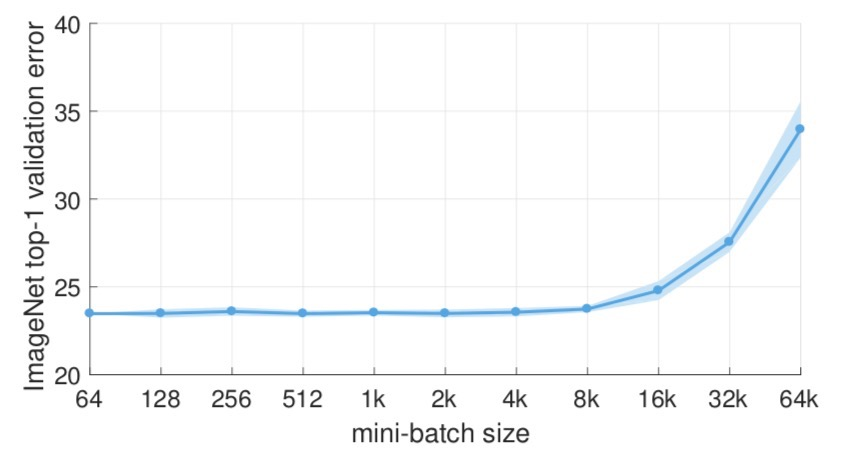
\includegraphics[width=12cm]{training1hour_result}
\caption{线性增大学习率和热启动方法下不同batch size下模型精度曲线}
\label{fig:training1hour_result}
\end{figure}
紧接着,伯克利尤洋等\upcite{train24min2017}提出分层自适应学习率算法。论文思想是不同网络层之间参数数值差距较大,而对应的梯度差距则更大,往往存在数量级之间的差距。作者指出不同网络层之间参数与梯度比值差距非常大,如果以相同的学习率来更新参数,必定造成较小参数更新步长过大,导致网络不收敛。故论文提出自适应各层参数大小的学习率调整方法,进一步将batch size由8k提升至32k,在24分钟内训完ImageNet。

随后,2018年Google Brain等\upcite{dontdecay2018}提出通过逐渐增大batch size替换学习率衰减的方法,最终将batch size提升至64k,只用两千五百多次迭代将ImageNet训到了理想精度。

\subsection{分布式深度学习中数据压缩的发展}
由2.1部分可知,分布式训练过程中同步通信量越小,分布式效率越高。近年来业界对在保证精度的情况下,如何尽可能地压缩传输梯度进行了相关研究。2017年,Xiangru Lian等\upcite{decentereasgd2017}提出去中心化的EASGD算法,减小网络通信量。在其环形拓扑结构中,每个worker只与其相邻的两个节点通信,将相邻两个节点的参数加和求平均,并求得本地参数与求得平均参数的差值更新至server。因为其更新的是参数的差值而不是参数本身,以此达到梯度压缩的目的。

2018年,Yujun Lin等\upcite{dgc2018}提出稀疏化梯度的方法。即每次只更新前0.1\%-1\%的梯度,极大减少了网络带宽,压缩比能达到600倍。剩下99.9\%未更新的梯度保留在本地,随着迭代的进行依次累加,直到该梯度达到前0.1\%~1\%后更新。论文解释这种将梯度保留在本地的方法,类似于增大batch size。提出动量修正,梯度修剪,动量因子隐蔽,热启动等方法保证压缩后梯度的精度和延迟更新梯度的影响。其中动量修正示意图如图~\ref{fig:dgc_picture}所示。
\begin{figure}[htp]
\centering
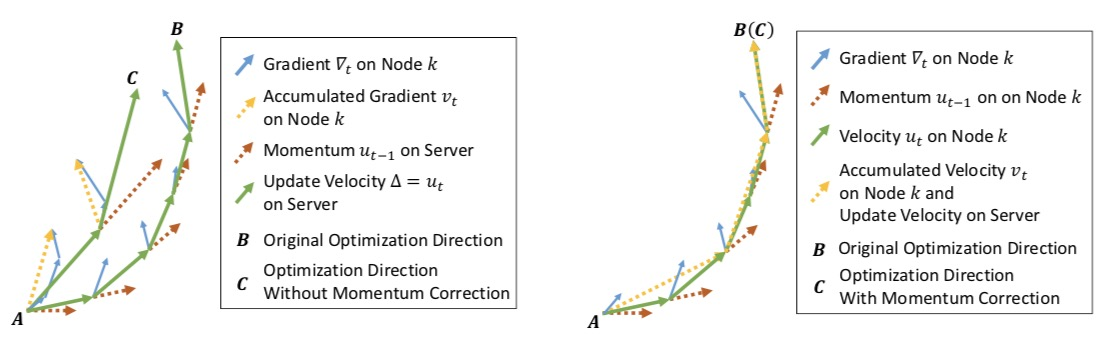
\includegraphics[width=14cm]{dgc_picture}
\caption{动量修正原理示意图}
\label{fig:dgc_picture}
\end{figure}

\section{本章小结}
本章主要介绍了分布式训练神经网络的特点,数据并行和模型并行这两种并行方法;介绍了神经网络在图像分类、物体检测、自然语言处理等领域的发展;最后详细介绍了分布式深度学习中涉及到的模型,系统,优化算法相关问题的研究进展。





\chapter{bf16数据同步方法}
本章首先阐述了本课题的研究背景及现实意义,然后介绍了国内外针对该问 题的研究与实现,说明了现有的解决方法及其存在的问题并根据这些问题提出了 本课题的研究内容。最后介绍了本论文的整体组织结构。
\section{引言}
介绍本章内容
正文内容
\section{框架设计}
如何在horovod上实现bf16
正文内容

\section{性能瓶颈}
带宽限制,用immintrin

\section{结果分析}
精度,性能(classification, detection, nlp)
\chapter{低精度梯度压缩方法}
受上一章节BF16更新算法启发,本章希望在不影响神经网络训练精度的情况下,尽可能减少梯度数据所需的比特位数,为进一步减少分布式通信开销提供数据压缩方法。本章将主要介绍梯度压缩的思路与实现方法,以及对应压缩方式在resnet50中的训练精度。通过resnet50最终的收敛精度判断相应压缩方法的有效性。
\section{引言}
根据第二章内容可知,分布式训练效率的高低主要取决于同步开销的大小,其主要取决于同步数据量的大小与网络带宽大小。在不影响训练精度的情况下,将梯度尽可能地压缩则可减少同步开销,提高分布式训练效率。本章将介绍探索梯度压缩方法的思路与具体实现方法,以及各个压缩方式下resnet50的最终收敛精度。

由第三章BF16分布式更新算法实现可知,基于horovod要实现新的数据压缩方法,则需在MPI中新增一个数据类型来解析该压缩数据,并实现一个该数据类型的求和函数供MPI调用。为快速验证本文提出的梯度压缩方法对神经网络训练精度的影响,本章提出的梯度压缩方法均通过对FP32浮点数或半精度浮点数对应比特位清零的方式来模拟对应的压缩方法。该模拟方法可避免对MPI的改动,使得本节提出的压缩方法能够快速得到验证。下面将对本节探索出的两种压缩方式进行详细介绍。
\section{9比特梯度压缩方法}
根据上一章BF16更新算法可知,BF16数据格式相对于原始FP32数据而言,去除了浮点数尾数中的后16比特位,仅保留7位有效比特位。本压缩算法根据这一思路,在BF16数据基础上,进一步减少尾数有效位,在保证训练精度情况下,尽可能减少尾数比特位,以减少分布式同步中的通信量。

\subsection{具体实现与实验结果}
\begin{figure}[htp]
\centering
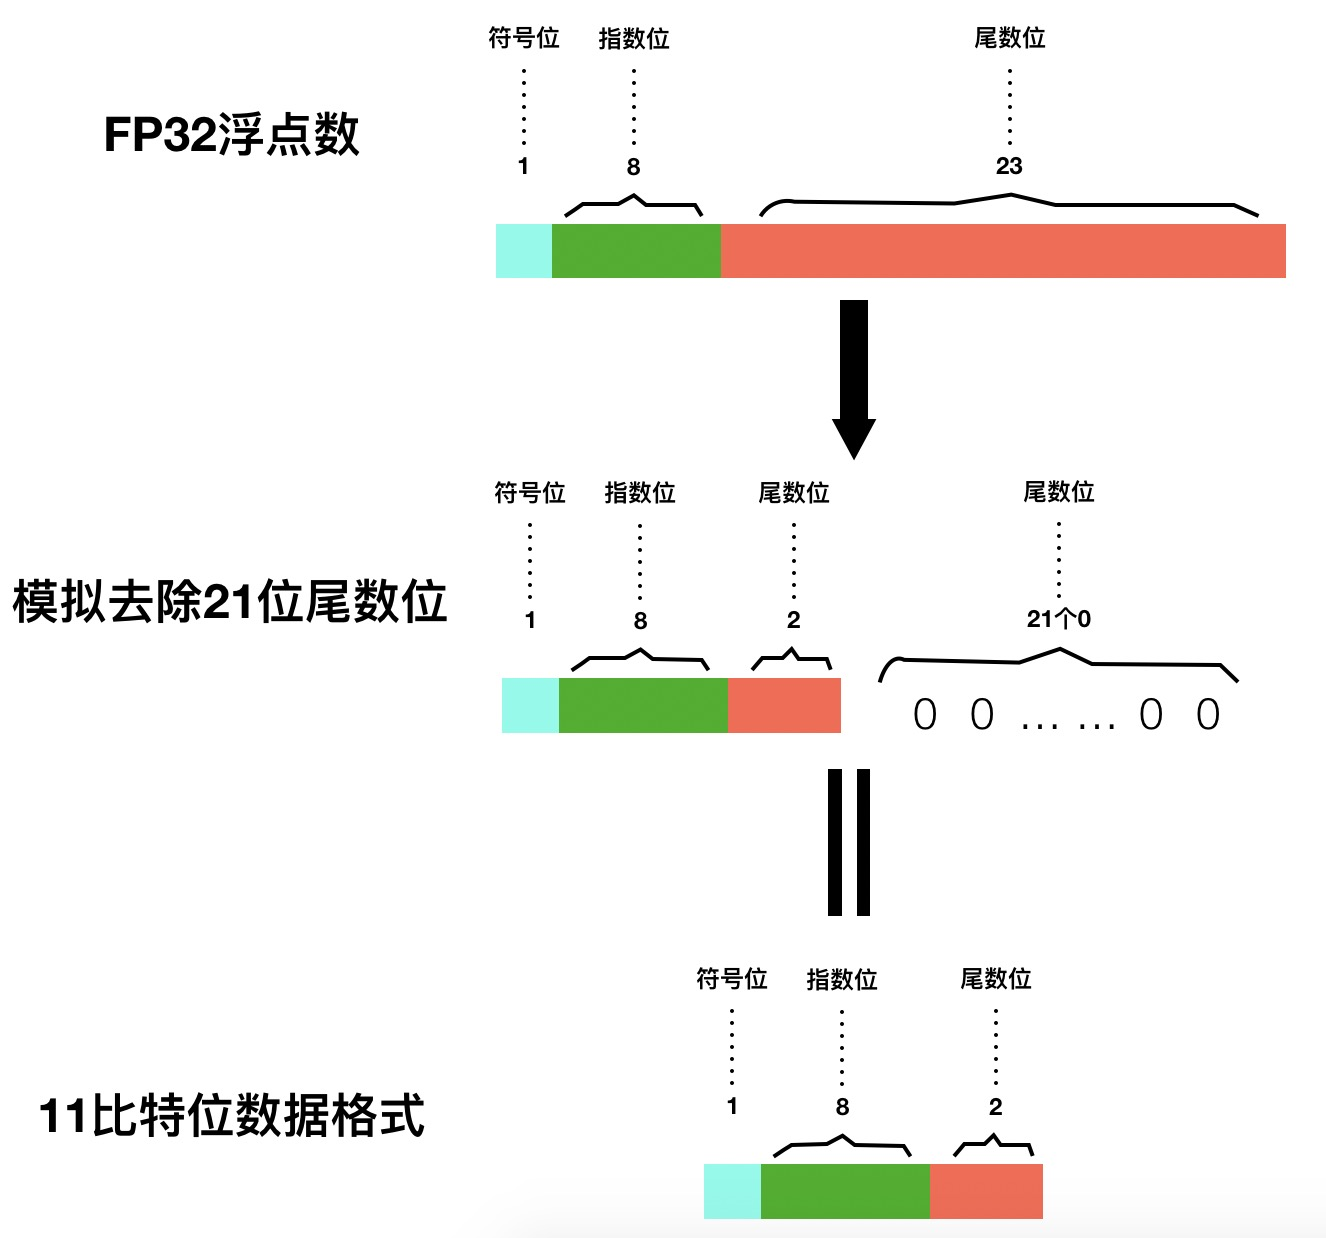
\includegraphics[width=10cm]{simulate_11bits}
\caption{模拟11比特数据表示示意图}
\label{fig:simulate_11bits}
\end{figure}
本节通过对原始FP32浮点数尾数位置零的方法模拟这种压缩方法。如在FP32浮点数基础上仅保留两位有效尾数位,形成11比特的数据格式,可通过将FP32浮点数的低21位清零达到相同效果,如图~\ref{fig:simulate_11bits}所示。

可知低21比特位清零后的浮点数等效于11比特位数据格式所表示数据。经实验验证:在同步梯度数据时仅保留两比特位的尾数情况下,神经网络也可收敛到原始浮点数梯度相同精度。在11比特有效位基础上,继续减少尾数位,保留1位尾数、去除所有尾数位情况下,在分类网上均能达到理想收敛精度。在去除所有尾数位仅使用9比特数据表示梯度情况下,resnet50的收敛曲线如图~\ref{fig:simulate_9bits_acc}所示。

\begin{figure}[htp]
\centering
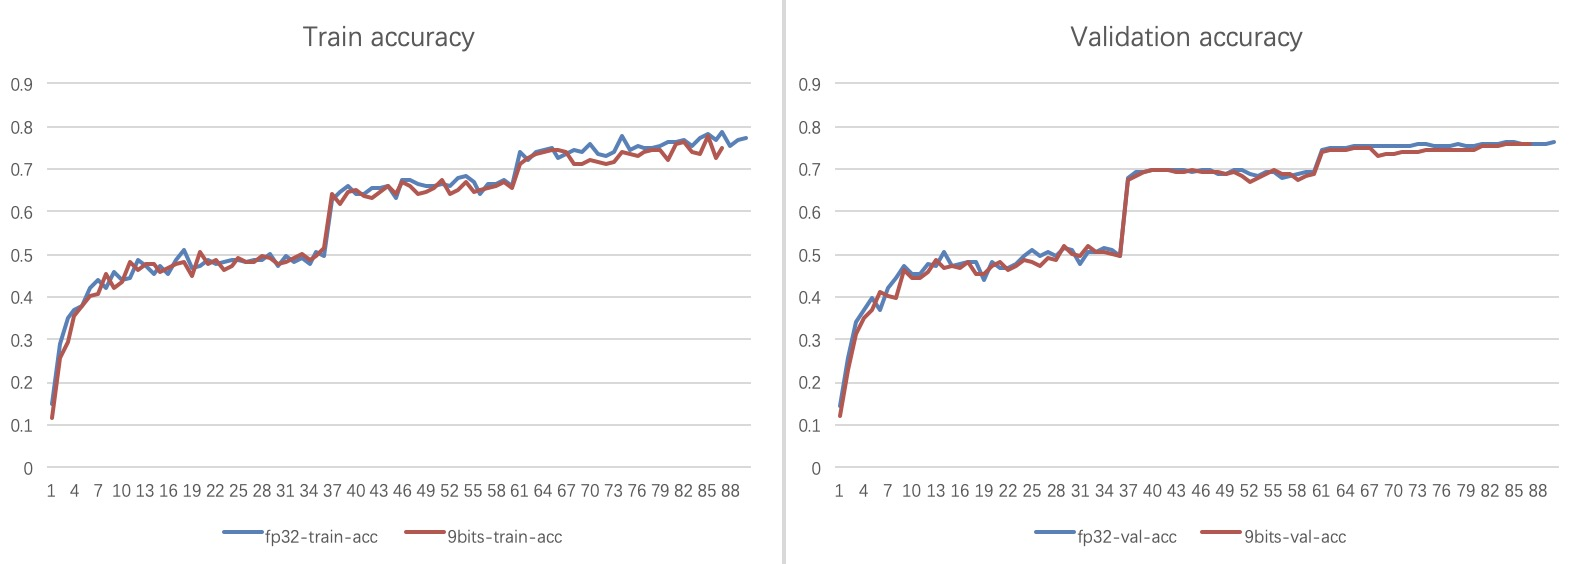
\includegraphics[width=10cm]{simulate_9bits_acc}
\caption{9比特梯度压缩方法与原始浮点数表示训练精度曲线}
\label{fig:simulate_9bits_acc}
\end{figure}

保留2位尾数,1位尾数,不保留尾数情况下,resnet50在验证集精度如表~\ref{tab:simulate_11_10_9bits_acc}所示。所有结果均在4节点8实例配置下训练得到。由表~\ref{tab:simulate_11_10_9bits_acc}可知,在原始浮点梯度基础上,仅保留2位尾数,1位尾数,不保留尾数情况下,网络精度与原始浮点数梯度精度相差<0.3\%。说明在误差允许范围内,在分类网中仅使用9比特数据(1个符号位,8个指数位)表示梯度即可满足训练精度要求,通过去除浮点数中所有尾数位的方法可在不影响神经网络训练精度前提下,减少分布式同步开销提升分布式训练性能。

\begin{table}[htb]
\centering
\noindent\begin{minipage}{0.45\textwidth}
\centering
\caption{不同尾数位下resnet50精度}
\label{tab:simulate_11_10_9bits_acc}
\begin{tabular}{p{2cm}p{2cm}}
\toprule[1.5pt]
有效尾数位 & 精度(\%) \\\midrule[1pt]
2 & 76.08 \\
1 & 76.01 \\
0 & 75.87 \\
\midrule[1pt]
\end{tabular}
\end{minipage}
\end{table}
本节提出的9比特梯度压缩方法还未在物体检测网中进行试验,下一步将在物体检测网络中使用该压缩方法进行分布式训练,以验证该9比特梯度数据压缩方法是否同样适用于物体检测网络。

\section{8比特梯度压缩方法}
由本文第二章可知,半精度浮点数也可用于训练神经网络,也能保证网络的训练精度与原始浮点数训练一致。半精度浮点数与BF16数据格式相比,少了3个指数位,仅5个指数位。根据上一节9比特梯度压缩方法可知,在仅保留2位,1位尾数或不保留尾数位情况下,均能保证神经网络训练精度与原始浮点数训练精度在误差允许范围内。本节结合半精度浮点数特点,本节提出8比特梯度压缩方法:在半精度浮点数基础上,去除16位半精度浮点数中低8位尾数,仅保留两个有效尾数位,使用8比特数据表示梯度,以此将梯度压缩成单字节数据。
\subsection{具体实现与实验分析}
为快速验证本节所提出的梯度压缩方法的有效性,本节通过将半精度浮点数特定尾数位清零的方式模拟该压缩方法。原理如图~\ref{fig:simulate_8bits}所示。在4节点8实例情况下,使用该方法将梯度数据压缩成单字节数据,resnet50的收敛曲线如图~\ref{fig:simulate_8bits_acc}所示。可知本节提出的8比特梯度压缩方法同样能达到原始训练精度:76.1\%,说明本节提出的压缩方法可在不影响神经网络精度情况下,减小分布式训练神经网络中的通信量,从而提升分布式训练效率。

\begin{figure}[htp]
\centering
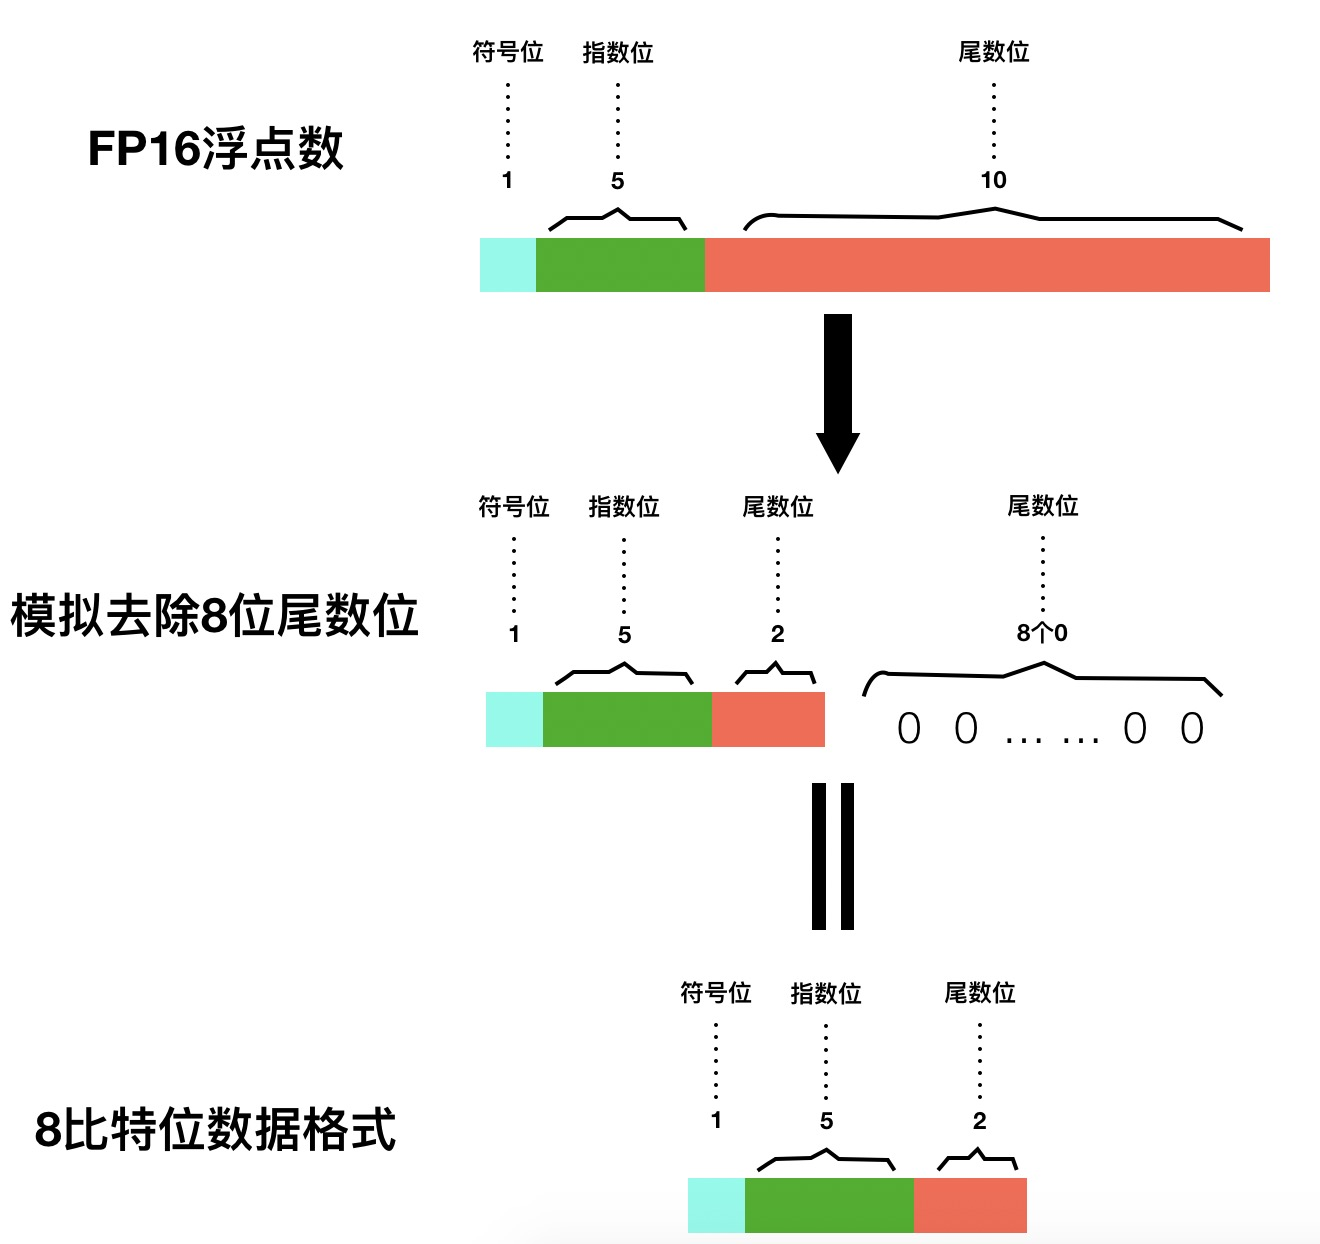
\includegraphics[width=10cm]{simulate_8bits}
\caption{模拟8比特数据表示示意图}
\label{fig:simulate_8bits}
\end{figure}

\begin{figure}[htp]
\centering
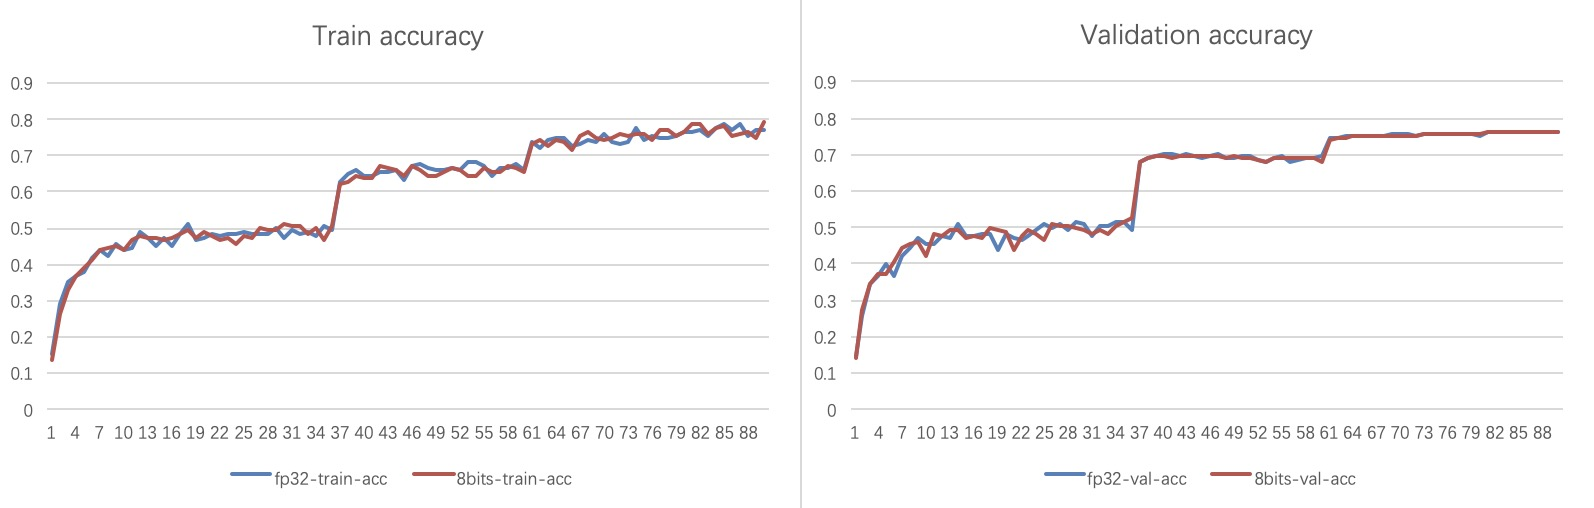
\includegraphics[width=10cm]{simulate_8bits_acc}
\caption{8比特位梯度压缩方法与原始浮点数表示训练精度曲线}
\label{fig:simulate_8bits_acc}
\end{figure}

同时,根据上一节提出的9比特压缩方法可知,可进一步在半精度浮点数上减少尾数位或去除所有尾数位,极限情况下仅使用6比特数据表示梯度。下一步将对该种可能的压缩方法进行尝试验证。也将在物体检测网络训练中应用本节提出的方法以说明该8比特压缩算法同样适用于物体检测网络。

\section{本章小结}
本章基于减少分布式训练神经网络通信开销的目的,希望通过减少梯度数据比特位的方法来减少通信数据量,提出9比特梯度压缩方法和8比特梯度压缩方法。经验证本章提出的两种压缩方法在resnet50网络中均能达到训练精度要求,说明这两种压缩方法的可行性。同时也指出下一步工作:将本章提出的两种压缩算法应用于物体检测网络,以说明这两种压缩算法对神经网络的普遍适用性。基于半精度浮点数提出的8比特位压缩方法还有压缩的空间,值得进一步尝试验证。








\chapter{总结与展望}
本章首先阐述了本课题的研究背景及现实意义,然后介绍了国内外针对该问 题的研究与实现,说明了现有的解决方法及其存在的问题并根据这些问题提出了 本课题的研究内容。最后介绍了本论文的整体组织结构。
\section{引言}
介绍本章内容
\chapter{绪论}
本章首先阐述了本课题的研究背景及现实意义,然后介绍了国内外针对该问 题的研究与实现,说明了现有的解决方法及其存在的问题并根据这些问题提出了 本课题的研究内容。最后介绍了本论文的整体组织结构。
\section{研究背景与意义}
正文内容

\subsection{(1.1.1 题目)}
正文内容

正文内容

\begin{figure}[htp]
\centering
\includegraphics{picmain}
\caption{图 1.1 名称}
\end{figure}

\subsubsection{(1.1.1.1 题目)}
正文内容

正文内容

正文内容

\subsubsection{(1.1.1.2 题目)}
正文内容

正文内容

正文内容

\subsection{(1.1.2 题目)}
正文内容

正文内容

\begin{figure}[htp]
\centering
\includegraphics{picmain}
\caption{图 1.2 名称}
\end{figure}

\section{研究现状}
正文内容
\subsection{分布式框架:ps,horovod介绍}
正文内容

\subsection{目前业界最新训练硬件:fp16,bf16训练}

\begin{table}[htp]
\centering
\caption{表 1.2 名称}
\begin{tabular}{|c|c|c|c|c|}
\hline
\makebox[2.07cm][0pt]{} & \makebox[2.07cm][0pt]{} & \makebox[2.07cm][0pt]{} & \makebox[2.07cm][0pt]{} & \makebox[2.07cm][0pt]{} \\
\hline
 & & & & \\
\hline
 & & & & \\
\hline
\end{tabular}
\end{table}

正文内容

正文内容

正文内容

正文内容

\section{本文工作}
正文内容

正文内容

正文内容

正文内容

正文内容

正文内容

\subsection{fp16训练}
正文内容

\begin{figure}[htp]
\centering
\includegraphics{picmain}
\caption{图 1.3 名称}
\end{figure}

\subsection{bf16训练}
正文内容

正文内容

\section{本文组织结构}

\begin{table}[htp]
\centering
\caption{表 1.2 名称}
\begin{tabular}{|c|c|c|c|c|}
\hline
\makebox[2.07cm][0pt]{} & \makebox[2.07cm][0pt]{} & \makebox[2.07cm][0pt]{} & \makebox[2.07cm][0pt]{} & \makebox[2.07cm][0pt]{} \\
\hline
 & & & & \\
\hline
 & & & & \\
\hline
\end{tabular}
\end{table}


\chapter{相关研究}
\label{chap:main}
\section{分布式训练神经网络的特点}
:1.精度,2.性能
\section{分布式深度学习系统的发展}
分布式论文:ng 2012年识别猫开始;
\section{混合精度训练发展,目前现有硬件不支持的问题}
本章将进入论文排版的正文, 按元素分主要包括:
{\kai 字体段落,图片表格,公式定理,参考文献}这几部分。
这个样例文件将包括模板中使用到的所有格式、模板中自定义命令到或者特有的东西,
都将被一一介绍,希望大家在排版自己的学位论文前能细致的看一遍,记住样例的格式和
方法,方便上手。

\section{字体段落}
\label{sec:font}

陈赓(1903年2月27日-1961年3月16日),原名陈庶康,中国湖南湘乡人,军事家。出生将门,其祖父为湘军将领陈翼怀。

Adobe中文字体有四种:

{\kai 楷体\verb|\kai|:陈赓,中国湖南湘乡人,军事家。出生将门,其祖父为湘军将领陈翼怀。%
1952年筹办并任人民解放军军事工程学院第一任院长兼政委,培养国防科技人才。1955年被授予大将军衔。}

{\fs 仿宋\verb|\fs|:陈赓,中国湖南湘乡人,军事家。出生将门,其祖父为湘军将领陈翼怀。%
1952年筹办并任人民解放军军事工程学院第一任院长兼政委,培养国防科技人才。1955年被授予大将军衔。}

{\hei 黑体\verb|\hei|:陈赓,中国湖南湘乡人,军事家。出生将门,其祖父为湘军将领陈翼怀。%
1952年筹办并任人民解放军军事工程学院第一任院长兼政委,培养国防科技人才。1955年被授予大将军衔。}

宋体就是正文字体了。下面测试字体大小,\LaTeX{}默认的列表环境会在
条目之间插入过多的行距,在下面这种情况可能正好,若用户需要
{\kai 正文行距}的列表环境,可以使用compactitem环境,记住这点很重要,不要再
用那种自己修改\verb|itemsep|的傻傻的办法了。
\begin{itemize}
\item[初号] {\song\chuhao 陈赓大将}
\item[小初] {\song\xiaochu 陈赓大将}
\item[一号] {\song\yihao 陈赓大将}
\item[小一] {\song\xiaoyi 陈赓大将}
\item[二号] {\song\erhao 陈赓大将}
\item[小二] {\song\xiaoer 陈赓大将}
\item[三号] {\song\sanhao 陈赓大将}
\item[小三] {\song\xiaosan 陈赓大将}
\item[四号] {\song\sihao 陈赓大将}
\item[小四] {\song\xiaosi 陈赓大将}
\item[五号] {\song\wuhao 陈赓大将}
\item[小五] {\song\xiaowu 陈赓大将}
\end{itemize}

\section{表格明细}
\label{sec:figure}
表格是论文的重要组成部分,我们从简单的表格讲起,到复杂的表格为止。

模板中关于表格的宏包有三个: \textsf{booktabs}、\textsf{array} 和
\textsf{longtabular}。三线表建议使用\textsf{booktabs}中提供的,
包含toprule、midrule 和 bottomrule三条命令,简单干脆!
它们与\textsf{longtable} 能很好的配合使用。下面来看一个表格实例:
\begin{table}[htb]
  \centering
  \begin{minipage}[t]{0.8\linewidth} % 如果想在表格中使用脚注,minipage是个不错的办法
  \caption[模板文件]{模板文件。如果表格的标题很长,那么在表格索引中就会很不美
    观,所以要像 chapter 那样在前面用中括号写一个简短的标题。这个标题会出现在索
    引中。}
  \label{tab:template-files}
    \begin{tabular*}{\linewidth}{lp{10cm}}
      \toprule[1.5pt]
      {\hei 文件名} & {\hei 描述} \\
      \midrule[1pt]
      nudtpaper.ins & \LaTeX{} 安装文件,docstrip\footnote{表格中的脚注} \\
      nudtpaper.dtx & 所有的一切都在这里面\footnote{再来一个}。\\
      nudtpaper.cls & 模板类文件。\\
      nudtpaper.cfg & 模板配置文。cls 和 cfg 由前两个文件生成。\\
      bstutf8.bst   & 参考文献 Bibtex 样式文件。\\
      mynudt.sty    & 常用的包和命令写在这里,减轻主文件的负担。\\
      \bottomrule[1.5pt]
    \end{tabular*}
  \end{minipage}
\end{table}

表 \ref{tab:template-files} 列举了本模板主要文件及其功能,基本上来说论文
中最可能用到的就是这种表格形式了。
请大家注意三线表中各条线对应的命令。这个例子还展示了如何在表格中正确使用脚注。
如果你不需要在表格中插入脚注,可以将minipage环境去掉。
由于\LaTeX{}本身不支持在表格中使用\verb|\footnote|,所以我们不得不将表格放在
小页中,而且最好将表格的宽度设置为小页的宽度,这样脚注看起来才更美观。

另外六院的同学在使用模板时需要使用一种固定宽度(往往是页宽,下面的例子由
rongdonghu提供)的表格,内容需要居中且可以自动调整。
解决办法是自定义了一种\verb|tabularx|中的\textbf{Z}环境,在论文模板中,
该命令已添加到\verb|mynudt.sty|中。下面是这种情况的实例:

\begin{table}[htbp]
\centering
\begin{minipage}[t]{0.9\linewidth}
\caption{Reed Solomon码的典型应用}
\label{tab:RSuse}
\begin{tabularx}{\linewidth}{cZ}
\toprule[1.5pt]
{\hei 应用领域} & {\hei 编码方案}\\
\midrule[1pt]
磁盘驱动器 & RS(32,28,5)码 \footnote{码长为32、维数为28、最小距离为5} \\
CD & 交叉交织RS码(CIRC) \\
DVD & RS(208,192,17)码、RS(182,172,11)码 \\
光纤通信 & RS(255,229,17)码 \\
\bottomrule[1.5pt]
\end{tabularx}
\end{minipage}
\end{table}

我们经常会在表格下方标注数据来源,或者对表格里面的条目进行解释。前面的脚注是一种
不错的方法,如果你不喜欢minipage方法的脚注。
那么完全可以在表格后面自己写注释,比如表~\ref{tab:tabexamp1}。
\begin{table}[htbp]
  \centering
  \caption{复杂表格示例 1}
  \label{tab:tabexamp1}
  \begin{minipage}[t]{0.8\textwidth} 
    \begin{tabularx}{\linewidth}{|l|X|X|X|X|}
      \hline
      \multirow{2}*{\backslashbox{x}{y}}  & \multicolumn{2}{c|}{First Half} & \multicolumn{2}{c|}{Second Half}\\
      \cline{2-5}
      & 1st Qtr &2nd Qtr&3rd Qtr&4th Qtr \\ 
      \hline
      \multirow{2}*{East$^{*}$} &   20.4&   27.4&   90&     20.4 \\
       &   30.6 &   38.6 &   34.6 &  31.6 \\ 
      West$^{**}$ &   30.6 &   38.6 &   34.6 &  31.6 \\ 
      \hline
    \end{tabularx}\\[2pt]
    \footnotesize
    *:东部\\
    **:西部
  \end{minipage}
\end{table}

此外,表~\ref{tab:tabexamp1} 同时还演示了另外三个功能:1)通过 \textsf{tabularx} 的
 \texttt{|X|} 扩展实现表格内容自动调整;2)通过命令 \verb|\backslashbox| 在表头部分
插入反斜线(WORD中很简单,但\LaTeX{}做表格需要一定的(极大的)想象力);3)就是
使用\verb|multirow|和\verb|multicolumn|命令。

不可否认 \LaTeX{} 的表格功能没有想象中的那么强大,不过只要你足够认真,足够细致,那么
同样可以排出来非常复杂非常漂亮的表格。可是科技论文中那么复杂表格有什么用呢?
上面那个表格就够用啦。

浮动体的并排放置一般有两种情况:1)二者没有关系,为两个独立的浮动体;2)二者隶属
于同一个浮动体。对表格来说并排表格既可以像表~\ref{tab:parallel1}、表~\ref{tab:parallel2} 
使用小页环境,也可以如表~\ref{tab:subtable}使用子表格来做。
图与表同出一源,后面我们将讲解子图(subfloat)的例子。
\begin{table}[htb]
\centering
\noindent\begin{minipage}{0.45\textwidth}
\centering
\caption{第一个并排子表格}
\label{tab:parallel1}
\begin{tabular}{p{2cm}p{2cm}}
\toprule[1.5pt]
111 & 222 \\\midrule[1pt]
222 & 333 \\\bottomrule[1.5pt]
\end{tabular}
\end{minipage}
\begin{minipage}{0.45\textwidth}
\centering
\caption{第二个并排子表格}
\label{tab:parallel2}
\begin{tabular}{p{2cm}p{2cm}}
\toprule[1.5pt]
111 & 222 \\\midrule[1pt]
222 & 333 \\\bottomrule[1.5pt]
\end{tabular}
\end{minipage}
\end{table}
\begin{table}[htbp]
\centering
\caption{并排子表格}
\label{tab:subtable}
\subfloat[第一个子表格]{
\begin{tabular}{p{2cm}p{2cm}}
\toprule[1.5pt]
111 & 222 \\\midrule[1pt]
222 & 333 \\\bottomrule[1.5pt]
\end{tabular}}\hskip2cm
\subfloat[第二个子表格]{
\begin{tabular}{p{2cm}p{2cm}}
\toprule[1.5pt]
111 & 222 \\\midrule[1pt]
222 & 333 \\\bottomrule[1.5pt]
\end{tabular}}
\end{table}

如果您要排版的表格长度超过一页,那么推荐使用\textsf{longtable}命令。
这里随便敲入一些无关的文字,使得正文看上去不是那么的少。
表~\ref{tab:performance} 就是 \textsf{longtable} 的简单示例。
\begin{longtable}[c]{c*{6}{r}}
\caption{实验数据}\label{tab:performance}\\
\toprule[1.5pt]
 测试程序 & \multicolumn{1}{c}{正常运行} & \multicolumn{1}{c}{同步}
& \multicolumn{1}{c}{检查点}   & \multicolumn{1}{c}{卷回恢复}
& \multicolumn{1}{c}{进程迁移} & \multicolumn{1}{c}{检查点} 	\\
& \multicolumn{1}{c}{时间 (s)} & \multicolumn{1}{c}{时间 (s)}
& \multicolumn{1}{c}{时间 (s)} & \multicolumn{1}{c}{时间 (s)}
& \multicolumn{1}{c}{时间 (s)} &  文件(KB)			\\
\midrule[1pt]%
\endfirsthead%

\multicolumn{7}{c}{续表~\thetable\hskip1em 实验数据}\\

\toprule[1.5pt]
 测试程序 & \multicolumn{1}{c}{正常运行} & \multicolumn{1}{c}{同步} 
& \multicolumn{1}{c}{检查点}   & \multicolumn{1}{c}{卷回恢复}
& \multicolumn{1}{c}{进程迁移} & \multicolumn{1}{c}{检查点} 	\\
& \multicolumn{1}{c}{时间 (s)} & \multicolumn{1}{c}{时间 (s)}
& \multicolumn{1}{c}{时间 (s)} & \multicolumn{1}{c}{时间 (s)}
& \multicolumn{1}{c}{时间 (s)} &  文件(KB)			\\
\midrule[1pt]%
\endhead%
\hline%

\multicolumn{7}{r}{续下页}%

\endfoot%
\endlastfoot%
CG.A.2 & 23.05   & 0.002 & 0.116 & 0.035 & 0.589 & 32491  \\
CG.A.4 & 15.06   & 0.003 & 0.067 & 0.021 & 0.351 & 18211  \\
CG.A.8 & 13.38   & 0.004 & 0.072 & 0.023 & 0.210 & 9890   \\
CG.B.2 & 867.45  & 0.002 & 0.864 & 0.232 & 3.256 & 228562 \\
CG.B.4 & 501.61  & 0.003 & 0.438 & 0.136 & 2.075 & 123862 \\
CG.B.8 & 384.65  & 0.004 & 0.457 & 0.108 & 1.235 & 63777  \\
MG.A.2 & 112.27  & 0.002 & 0.846 & 0.237 & 3.930 & 236473 \\
MG.A.4 & 59.84   & 0.003 & 0.442 & 0.128 & 2.070 & 123875 \\
MG.A.8 & 31.38   & 0.003 & 0.476 & 0.114 & 1.041 & 60627  \\
MG.B.2 & 526.28  & 0.002 & 0.821 & 0.238 & 4.176 & 236635 \\
MG.B.4 & 280.11  & 0.003 & 0.432 & 0.130 & 1.706 & 123793 \\
MG.B.8 & 148.29  & 0.003 & 0.442 & 0.116 & 0.893 & 60600  \\
LU.A.2 & 2116.54 & 0.002 & 0.110 & 0.030 & 0.532 & 28754  \\
LU.A.4 & 1102.50 & 0.002 & 0.069 & 0.017 & 0.255 & 14915  \\
LU.A.8 & 574.47  & 0.003 & 0.067 & 0.016 & 0.192 & 8655   \\
LU.B.2 & 9712.87 & 0.002 & 0.357 & 0.104 & 1.734 & 101975 \\
LU.B.4 & 4757.80 & 0.003 & 0.190 & 0.056 & 0.808 & 53522  \\
LU.B.8 & 2444.05 & 0.004 & 0.222 & 0.057 & 0.548 & 30134  \\
EP.A.2 & 123.81  & 0.002 & 0.010 & 0.003 & 0.074 & 1834   \\
EP.A.4 & 61.92   & 0.003 & 0.011 & 0.004 & 0.073 & 1743   \\
EP.A.8 & 31.06   & 0.004 & 0.017 & 0.005 & 0.073 & 1661   \\
EP.B.2 & 495.49  & 0.001 & 0.009 & 0.003 & 0.196 & 2011   \\
EP.B.4 & 247.69  & 0.002 & 0.012 & 0.004 & 0.122 & 1663   \\
EP.B.8 & 126.74  & 0.003 & 0.017 & 0.005 & 0.083 & 1656   \\
\bottomrule[1.5pt]
\end{longtable}

另外,有的同学不想让某个表格或者图片出现在索引里面,那么请使用命令 \verb|\caption*{}|,
这个命令不会给表格编号,也就是出来的只有标题文字而没有“表~XX”,“图~XX”,否则
索引里面序号{\kai 不连续}就显得不伦不类,这也是 \LaTeX{} 里星号命令默认的规则。

\section{绘图插图}

本模板不再预先装载任何绘图包(如 \textsf{pstricks,pgf} 等),完全由你自己来决定。
个人觉得 \textsf{pgf} 不错,不依赖于 Postscript。此外还有很多针对 \LaTeX{} 的
 GUI 作图工具,如 XFig(jFig), WinFig, Tpx, Ipe, Dia, Inkscape, LaTeXPiX,
jPicEdt 等等。本人强烈推荐\textsf{Ipe}。

一般图形都是处在浮动环境中。之所以称为浮动是指最终排版效果图形的位置不一定与源文
件中的位置对应,这也是刚使用 \LaTeX{} 同学可能遇到的问题。
如果要强制固定浮动图形的位置,请使用 \textsf{float} 宏包,
它提供了 \texttt{[H]}(意思是图片就给我放在这里\textcolor{red}{H}ere)参数,
但是除非特别需要,不建议使用\texttt{[H]},而是推荐使用\texttt{[htbp]},
给\LaTeX{}更多选择。比如图~\ref{fig:ipe}。
\begin{figure}[htbp] % use float package if you want it here
  \centering
  \includegraphics[width=3in]{hello}
  \caption{利用IPE制图}
  \label{fig:ipe}
\end{figure}

若子图共用一个计数器,
那么请看图~\ref{fig:big1},它包含两个小图,分别是图~\ref{fig:subfig1} 
和图~\ref{fig:subfig2}。这里推荐使用\verb|\subfloat|,{\bf 不要再用}
\verb|\subfigure|和\verb|\subtable|。
\begin{figure}[htb]
  \centering%
  \subfloat[第一个小图形]{%
    \label{fig:subfig1}
    \includegraphics[height=2cm]{xh}}\hspace{4em}%
  \subfloat[第二个小图形。如果标题很长的话,它会自动换行,这个 caption 就是这样的例子]{%
    \label{fig:subfig2}
    \includegraphics[height=2cm]{xhh}}
  \caption{包含子图形的大图形}
  \label{fig:big1}
\end{figure}

而下面这个例子显示并排$3\times2$的图片,见图\ref{fig:subfig:3x2}:
\begin{figure}[htb]
\centering
\subfloat[]{\includegraphics[width=.27\textwidth]{typography}} \qquad
\subfloat[]{\includegraphics[width=.27\textwidth]{typography}} \qquad
\subfloat[]{\includegraphics[width=.27\textwidth]{typography}} \qquad
\subfloat[]{\includegraphics[width=.27\textwidth]{typography}} \qquad
\subfloat[]{\includegraphics[width=.27\textwidth]{typography}} \qquad
\subfloat[]{\includegraphics[width=.27\textwidth]{typography}}
\caption{并排图片}
\label{fig:subfig:3x2}
\end{figure}

要注意,图\ref{fig:subfig:3x2}例中
\texttt{qquad}相当于\verb|\hspace{2em}|,也就是2个字符的宽度,约0.08倍页宽,
图片宽度设定为0.27倍页宽是合适的;在该环境中,尽量不要手动换行,所以,不妨自己计算一下!

如果要把编号的两个图形并排,那么小页(minipage)就非常有用了,可以分别参考
图\ref{fig:parallel1}和图\ref{fig:parallel2}。其实这个例子和表格一节中并排
放置的表格一摸一样。
\begin{figure}[htb]
\begin{minipage}{0.48\textwidth}
  \centering
  \includegraphics[height=1.2cm]{xhh}
  \caption{并排第一个图}
  \label{fig:parallel1}
\end{minipage}\hfill
\begin{minipage}{0.48\textwidth}
  \centering
  \includegraphics[height=1.2cm]{xhh}
  \caption{并排第二个图}
  \label{fig:parallel2}
\end{minipage}
\end{figure}

图形就说这么多,因为大家在写论文是遇到的最大问题不是怎么把图插进去,
而是怎样做出专业的、诡异的、震撼的图片来,记得在这时参考前面推荐的那
些工具吧,当然必不可少的是Matlab了,至于如何加入中文标注、支持中文等等
可以上网去查,但这里{\kai 推荐一点},用好export命令,使得插入图片时尽可能的不要
缩放,保证图文的一致性。

\section{公式定理}
\label{sec:equation}
贝叶斯公式如式~(\ref{equ:chap1:bayes}),其中$p(y|\mathbf{x})$为后验;
$p(\mathbf{x})$为先验;分母$p(\mathbf{x})$ 为归一化因子,这是
实际应用中十分恐怖的一个积分式。
\begin{equation}
\label{equ:chap1:bayes}
p(y|\mathbf{x}) = \frac{p(\mathbf{x},y)}{p(\mathbf{x})}=
\frac{p(\mathbf{x}|y)p(y)}{p(\mathbf{x})} 
\end{equation}

论文里面公式越多,\TeX{} 就越 happy。再看一个 \textsf{amsmath} 的例子:
\newcommand{\envert}[1]{\left\lvert#1\right\rvert} 
\begin{equation}\label{detK2}
\det\mathbf{K}(t=1,t_1,\dots,t_n)=\sum_{I\in\mathbf{n}}(-1)^{\envert{I}}
\prod_{i\in I}t_i\prod_{j\in I}(D_j+\lambda_jt_j)\det\mathbf{A}
^{(\lambda)}(\overline{I}|\overline{I})=0.
\end{equation} 

大家在写公式的时候一定要好好看\textsf{amsmath}的文档,并参考模板中的用法:
\begin{multline*}%\tag{[b]} % 这个出现在索引中的
\int_a^b\biggl\{\int_a^b[f(x)^2g(y)^2+f(y)^2g(x)^2]
 -2f(x)g(x)f(y)g(y)\,dx\biggr\}\,dy \\
 =\int_a^b\biggl\{g(y)^2\int_a^bf^2+f(y)^2
  \int_a^b g^2-2f(y)g(y)\int_a^b fg\biggr\}\,dy
\end{multline*}

再看\ref{equ:split}:
\begin{equation}\label{equ:split}
\begin{split}
C(z) &= [z^n] \biggl[\frac{e^{3/4}}{\sqrt{1-z}} +
e^{-3/4}(1-z)^{1/2} + \frac{e^{-3/4}}{4}(1-z)^{3/2}
+ O\Bigl( (1-z)^{5/2}\Bigr)\biggr] \\
&= \frac{e^{-3/4}}{\sqrt{\pi n}} - \frac{5e^{-3/4}}{8\sqrt{\pi
n^3}} + \frac{e^{-3/4}}{128 \sqrt{\pi n^5}} +
O\biggl(\frac{1}{\sqrt{\pi
n^7}}\biggr)
\end{split}
\end{equation}

当然了,数学中必不可少的是定理和证明:
\begin{theorem}
  \label{chapTSthm:rayleigh solution}
  假定 $X$ 的二阶矩存在:
  \begin{equation}
         O_R(\mathbf{x},F)=\sqrt{\frac{\mathbf{u}_1^T\mathbf{A}\mathbf{u}_1} {\mathbf{u}_1^T\mathbf{B}\mathbf{u}_1}}=\sqrt{\lambda_1},
  \end{equation}
  其中 $\mathbf{A}$ 等于 $(\mathbf{x}-EX)(\mathbf{x}-EX)^T$,$\mathbf{B}$ 表示协方差阵 $E(X-EX)(X-EX)^T$,$\lambda_1$
$\mathbf{u}_1$是$\lambda_1$对应的特征向量,
\end{theorem}

对于希腊符号使用\verb|mathbf|命令可能有些问题,所以建议对符号
用\verb|bm|加粗,记得用\verb|\up<greek>|切换正体符号,下面看几个例子:
\verb|\gamma|斜体代表变量$\gamma$,\verb|\bm{\upgamma}|正体代表向量$\bm{\upgamma}$,
。\verb|\Gamma|正体代表操作符号$\Gamma$,
\verb|\bm{\Gamma}|正体粗体代表矩阵形式$\bm{\Gamma}$,
\verb|\varGamma|斜体代表变量$\varGamma$。另外对于大小写斜体的加粗可以见$\bm{\gamma}$和$\bm{\varGamma}$,
但是这两种科技论文中很少出现,这里只做测试。
非符号普通向量就用\verb|\mathbf|吧:$\mathbf{x}_k,\mathbf{X}_k$。
完整测试如下$\omega,\bm{\omega},\upomega,\bm{\upomega},\Omega,\bm{\Omega},\varOmega,\bm{\varOmega}$。

\begin{proof}
上述优化问题显然是一个Rayleigh商问题。我们有
  \begin{align}
     O_R(\mathbf{x},F)=\sqrt{\frac{\mathbf{u}_1^T\mathbf{A}\mathbf{u}_1} {\mathbf{u}_1^T\mathbf{B}\mathbf{u}_1}}=\sqrt{\lambda_1},
 \end{align}
 其中 $\lambda_1$ 下列广义特征值问题的最大特征值:
$$
\mathbf{A}\mathbf{z}=\lambda\mathbf{B}\mathbf{z}, \mathbf{z}\neq 0.
$$
 $\mathbf{u}_1$ 是 $\lambda_1$对应的特征向量。结论成立。
\end{proof}

下面来看看算法环境的定义和使用。
我们知道,故障诊断的最终目的,是将故障定位到部件,而由于信号--部件依赖矩阵的存在,因此,实质性的工作是找出由故障部件发出异常信号,
不妨称为源异常信号,而如前所述,源异常信号与异常信号依赖矩阵$\mathbf{S_a}$的全零列是存在一一对应的关系的。因此,我们只要获得了$\mathbf{S_a}$的全零列的相关信息,
也就获得了源异常信号的信息,从而能进一步找到故障源。
通过以上分析,我们构造算法\ref{alg53},用于实现非回路故障诊断。
\begin{algorithm}[htbp]
  \caption{非回路故障诊断算法}
  \label{alg53}
  \begin{algorithmic}[1]
    \REQUIRE 信号--部件依赖矩阵$\mathbf{A}$,信号依赖矩阵$\mathbf{S}$,信号状态向量$\alpha$
    \ENSURE 部件状态向量$\gamma$
    \STATE $\mathbf{P}\leftarrow\left(<\alpha>\right)$
    \STATE $\mathbf{S_{a}}\leftarrow\mathbf{P^T}\mathbf{S}\mathbf{P}$
    \FOR{$i=1$ to $S_a$的阶数$m$}
    \STATE $s_i\leftarrow s_i$的第$i$个行向量
    \ENDFOR
    \STATE $\beta_a\leftarrow\lnot \left(s_1\lor s_2\lor \cdots\lor s_m\right)^T$
    \STATE $\beta\leftarrow\mathbf{P}\beta_a$
    \STATE $\gamma\leftarrow\mathbf{A}\beta$
  \end{algorithmic}
\end{algorithm}

第一类故障回路推理与非回路故障推理是算法基本相同,稍微不同的是$\beta_a$的计算。因为第一类故障回路中的信号全部可能是源异常信号,因此我们不必计算
$\beta_a=\lnot \left(\left[s_1\lor s_2\lor \cdots\lor s_m\right]^T\right)$,而直接取$\beta_a=\underbrace{\left[\begin{array}{cccc}1&1&\cdots&1\end{array}\right]^T}_m$,将$\beta_a$代入
算法\ref{alg53},有
\[\beta=\mathbf{P}\beta_a=\mathbf{P}\underbrace{\left[\begin{array}{cccc}1&1&\cdots&1\end{array}\right]^T}_m=\alpha\]
因此一类故障回路的推理算法变得相当简单,例如算法\ref{alg54}
\begin{algorithm}[htbp]
  \caption{第一类故障回路诊断算法}
  \label{alg54}
  \begin{algorithmic}[1]
    \REQUIRE 信号--部件依赖矩阵$\mathbf{A}$,信号状态向量$\alpha$
    \ENSURE 部件状态向量$\gamma$
    \STATE $\gamma\leftarrow\mathbf{A}\alpha$
  \end{algorithmic}
\end{algorithm}

\section{参考文献}
\label{sec:bib}
当然参考文献可以直接写 bibitem,虽然费点功夫,但是好控制,各种格式可以自己随意改
写,在nudtpaper里面,建议使用JabRef编辑和管理文献,再结合\verb|bstutf8.bst|,
对中文的支持非常不错,格式也很规范。

本模板推荐使用 BIB\TeX,样式文件为 bstutf8.bst,符合学校的参考文献格式(如专利
等引用未加详细测试)。看看这个例子,关于书的\upcite{tex, companion},
还有这些\upcite{Krasnogor2004e, clzs, zjsw},关于杂志的\upcite{ELIDRISSI94,
  MELLINGER96, SHELL02},硕士论文\upcite{zhubajie, metamori2004},博士论文
\upcite{shaheshang, FistSystem01},标准文件\upcite{IEEE-1363},会议论文\upcite{DPMG,kocher99,alexnet2012},%
技术报告\upcite{NPB2}。中文参考文献\upcite{cnarticle}\textsf{特别注意},需要在\verb|bibitem|中
增加\verb|language|域并设为\verb|zh|,英文此项可不填,之后由\verb|bstutf8|统一处理
(具体就是决定一些文献在中英文不同环境下的显示格式,如等、etc)。
若使用\verb|JabRef|,则你可按下面步骤来设置:
选择\textsf{Options}$\rightarrow$\textsf{Set Up General Fields},
在\verb|General:|后加入\verb|language|就可以了。

有时候不想要上标,那么可以这样 \cite{shaheshang},这个非常重要。

\section{代码高亮}
有些时候我们需要在论文中引入一段代码,用来衬托正文的内容,或者体现关键思路的实现。
在模板中,统一使用\texttt{listings}宏包,并且设置了基本的内容格式,并建议用户只
使用三个接口,分别控制:编程语言,行号以及边框。简洁达意即可,下面分别举例说明。

首先是设定语言,来一个C的,使用的是默认设置:
\begin{lstlisting}[language=C]
void sort(int arr[], int beg, int end)
{
  if (end > beg + 1)
  {
    int piv = arr[beg], l = beg + 1, r = end;
    while (l < r)
    {
      if (arr[l] <= piv)
        l++;
      else
        swap(&arr[l], &arr[--r]);
    }
    swap(&arr[--l], &arr[beg]);
    sort(arr, beg, l);
    sort(arr, r, end);
  }
}
\end{lstlisting}

当我们需要高亮Java代码,不需要行号,不需要边框时,可以:
\begin{lstlisting}[language=Java,numbers=none,frame=none]
// A program to display the message
// "Hello World!" on standard output

public class HelloWorld {
 
   public static void main(String[] args) {
      System.out.println("Hello World!");
   }
      
}   // end of class HelloWorld
\end{lstlisting}

细心的用户可能发现,行号被放在了正文框之外,事实上这样是比较美观的,
如果有些用户希望在正文框架之内布置所有内容,可以:
\begin{lstlisting}[language=perl,xleftmargin=2em,framexleftmargin=1.5em]
#!/usr/bin/perl
print "Hello, world!\n";
\end{lstlisting}

好了,就这么多,\texttt{listings}宏包的功能很强大也很复杂,如果需要自己定制,
可以查看其手册,耐心阅读总会找到答案。
\textbf{注意:} 当前代码环境中文注释的处理还不是很完善,对于注释请妥善处理。
在本模板中,推荐算法环境或者去掉中文的listings代码环境。
如果需要包含中文注释,不要求代码高亮,
就用\texttt{code}环境,这个环境是Verbatim的定制版,简单有效,
调用的是fancyvbr宏包,用户可在mynudt.sty中修改它的外观等等。
这里我们还可以给代码加上标签。
\begin{code}[label=hello.c]
public class HelloWorld {
   public static void main(String[] args) {
      System.out.println("Hello World!");
   }
}   // 世界,你好!
\end{code}

\section{符号列表}

{\hei 前面的话:}{\kai\color{blue} 
2.2版本后默认使用nomencl环境,如果你还是希望使用传统的\verb|definition.tex|,那么只需注释掉
顶层文件中的nomenclature即可。}

符号列表使用的是\verb|nomencl|包,自己简单定制了下,使用方法分为四步:
\begin{compactenum}
\item 将\verb|\makenomenclature|语句放在正文前,即\verb|\begin{document}|前面;
\item 将\verb|\printnomenclature|放在论文中,我在例子中将符号列表放在了英文摘要的
后面,正文第一章的前面,当然,你可以根据自己的需要或者教研室的规范放置在合理的位置上,
为了页面引用的正确,在这句话前面放上\verb|\cleardoublepage|;
\item 使用\verb|\nomenclature|命令在论文的各个位置上添加符号定义,语法后面会讲到;
\item 编译。编译需要首先运行一遍xelatex,之后运行
\begin{code}
makeindex -s nomencl.ist -o thesis.nls thesis.nlo
\end{code}
\end{compactenum}

你可以把这句编译命令放在\verb|makepdf.bat|中第一个\verb|xelatex thesis|下面。然后
双击\verb|makepdf.bat|就可以了,论文模板中已经为你添加上了,如果你强烈不想使用
nomencl环境,只要把它注释掉(前面加\verb|rem|)就可以。
另外,由于我使用的是VIM来编辑\TeX{}代码,具体到每个编辑器(诸如WinEDT,TeXWorks等)
如何设定该命令的快捷按钮,诸位可以搜索网上的教程。

下面简单说明下\verb|\nomenclature|命令,语法为。这里插入一些随机的文字,希望
对你在阅读帮助中的思维没有什么不良的影响。
\begin{code}
\nomenclature[<prefix>]{<symbol>}{<desc>}{<null>}
\end{code}
\verb|nomencl|模板的默认排序方法可能(大多都)不满足要求,
论文模板里,我们通过设定\verb|<prefix>|来实现符号列表的排序。
它分为两部分,比如如\verb|[Aa]|,第一个字母的含义是:
\begin{compactitem}
\item[`A'] 符号归为拉丁字母
\item[`G'] 希腊字母
\item[`X'] 上标
\item[`Z'] 下标
\end{compactitem}
每个标识后边的字幕\verb|a-z|作为当前符号组内的排列顺序,比如$\beta$就可以写成
\verb|[Gb]|,诸如此类。当然你一定注意到了,这个排序分组的设定只是为了记忆
方便,并不是强制的,因此你可以有自己的方案,比如Z是Greek,
R是Roman什么的,只要统一就好,只需记住,组间排列是按字母顺序排的。

注意符号表分四列,前三列的含义与命令中相同,
最后一列是符号定义时所在的页码。效果看例子,对于下式:
\begin{equation}\label{eq:heatflux}
   \dot{Q} = k \cdot A \cdot \Delta T
\end{equation}%
\nomenclature[Aq]{$\dot{Q}$}{heat flux}{}%
\nomenclature[Ak]{$k$}{overall heat transfer coefficient,式\eqref{eq:ohtc}}{}%
\nomenclature[Aa]{$A$}{area}{}%
\nomenclature[Al]{$L$}{length}{}%
\nomenclature[At]{$T$}{temperature}{}%
\nomenclature[At]{$\Delta T$}{temperature difference}{}%
\nomenclature[Gr]{$\gamma$}{中文测试, 以及一句很长的物理意义,很有可能超过当前栏的宽度,主要目的是看一看会不会出现某些异常情况。}{}%

或者:
\begin{equation}\label{eq:ohtc}
    \frac{1}{k} = \left[\frac{1}{\alpha _{\mathrm{i}}\,r_{\mathrm{i}}} +
    \sum^n_{j=1}\frac{1}{\lambda _j}\,
    \ln \frac{r_{\mathrm{a},j}}{r_{\mathrm{i},j}} +
    \frac{1}{\alpha _{\mathrm{a}}\,
    r_{\mathrm{a}}}\right] \cdot r_{\mathrm{reference}}
\end{equation}%
\nomenclature[Ga]{$\alpha$}{convection heat transfer coefficient}{}%
\nomenclature[Zi]{i}{in}{}%
\nomenclature[Gl]{$\lambda$}{thermal conductivity}{}%
\nomenclature[Za]{a}{out}{}%
\nomenclature[Zn]{$n$}{number of walls}{}%
\nomenclature[Zj]{$j$}{running parameter}{}%

{\hei 注意事项:}{\kai 模板中定制的nomencl格式在mynudt.sty中,默认是三栏的,分别是:
``符号'',``定义'',``首次出现页码'',
注意这里的符号列表都没有单位,如果你需要额外的栏输入单位(呵呵,聪明的读者可能看出来
了,\verb|nomenclature|命令最后一个是空的,就是用来让你赋予她各种意义的)。
此时就需要你有一点点动手能力了(其实只要会修改表格就行),
方法很简单,比如需要添加``国际单位制''这一栏,则
\begin{compactenum}
\item 论文中\verb|\nomenclature|命令的第三个参数就让他代表单位,也可留空;
\item 将\verb|mynudt.sty|中longtable的表头添加``国际单位制''几个字,
你也可以取其他的名字,放在那个{\kai 应该出现的}位置上;
\item 由于增加了5个字,就把前面栏的宽度数字减5,同时设定第三栏宽度为5,
注意这一步需要你自己调整,记得不要让表格超出边界就行。
\end{compactenum}
}

\section{中文习惯}
\label{sec:chinese}

对于itermize过大的行间距,用户可以使用compactitem环境来替代,但是模板中不进行默认替代,
因为只有用户真正发现列表不好看才会找到这里,而且在示例文件中,
陈赓大将那个列表环境如果压缩了行距会很不好看。谢谢ZhangLei的建议!

{\hei 一个重要的提示:}
作者自己的定义命令、包等,不要放在模板里面,请放到\verb|mynudt.sty|
中,这样模板时,只要覆盖\verb|nudtpaper.cls|即可。

中文破折号为一个两个字宽垂直居中的直线,输入法直接得到的破折号是两个断开的小短线
(——),这看起来不舒服。所以模板中定义了一个破折号的命令 \verb|\pozhehao|,请看:

厚德博学,强军兴国\hfill \pozhehao{}国防科大校训




%%% Local Variables:
%%% mode: latex
%%% TeX-master: "../main"
%%% End:

\begin{ack}
  光阴荏苒、岁月如梭,转眼间在国防科学技术大学学习已经两年有余,美好的研究生生涯即将结束。在这两年多的时间里,很幸运有诸多老师,同学,朋友的陪伴。在学习上遇到困难时能及时给予我帮助,启发我进一步思考,为我提供了如此快乐,充实的学习生活;在生活上遇到问题时能及时为我开导,帮助我从消极情绪中快速走出来,让我一直以积极,乐观的心态面对各种困难。毕业在即,我要向所有给予我指导和帮助的老师、同学、朋友以及家人表示衷心的感谢!
  
  特别感谢我的指导老师李东升研究员。李老师学识渊博,和蔼可亲,在我还没正式步入研究生生涯时就给予了我很多帮助,解答我的疑惑,给我学习资料,安排师兄带我学习,使我尽早地进入了研究生生活,融入实验室大家庭。研究生期间李老师总是尽可能地满足我个人的研究兴趣并加以指导,感谢老师给我们提供了如此自由、良好的学习氛围。
  
  衷心感谢张钊宁老师。是张老师把我领进了深度学习的大门。在他的指导下,我做了许多有意义工作,也让自己的能力有了很大的提升。张老师也是我们的师兄,学习生活上有任何问题,困惑都可以从朋友的角度跟他反应交流。感谢张老师在我对毕设方向有疑惑动摇以及对未来工作担心时,及时和我沟通,帮我推荐工作。在张老师的指导、帮助下,使我的科研、动手能力有了很大提升,也让我对未来工作更加自信。
  
  衷心感谢intel公司赵鹏老师以及组内同事在我做毕设时给予我的帮助。在我对某一方面知识有疑问时,赵老师总是找相关领域的工作人员为我解答疑问;在我毕设遇到问题时,及时帮我分析问题,指明我的方向。感谢赵老师和Jason在我的毕设和组内任务有冲突时,以我毕设为主,让我有足够的时间完成毕设。衷心感谢同事们在我有疑问时为我清晰解答相关问题,在你们的帮助下让我得以完成毕设内容,也让我对相关领域知识有了深入了解。
  
  感谢实验室其他指导老师:彭宇行老师,王意洁老师,张一鸣老师,沈思琪老师,你们的研究态度和对科研的追求,是我们学习的榜样。感谢实验室师兄师姐:尹璐伽,彭宝云,赵云祥,陈心圆,黎敏讷,陈圣灵,李真真等和众多同级的小伙伴:秦政,于昊,卢孟龙,左钟融,徐军,邵旭颖以及其他师弟师妹们在学习,生活中给予的帮助,你们的陪伴使得实验室的科研氛围充满了快乐。另外还要感谢PDL实验室的工作人员,你们对我学习之外的诸多事宜给予了充分的支持。

\end{ack}


\cleardoublepage
\phantomsection
\addcontentsline{toc}{chapter}{参考文献}
\bibliographystyle{bstutf8}
\bibliography{ref/myrefs}

\begin{resume}

  \section*{发表的学术论文} % 发表的和录用的合在一起

  \begin{enumerate}[label={[\arabic*]}]
  \addtolength{\itemsep}{-.36\baselineskip}%缩小条目之间的间距,下面类似
  %\item Yang Y, Ren T L, Zhang L T, et al. Miniature microphone with silicon-based ferroelectric thin films. Integrated Ferroelectrics, 2003,52:229-235. (SCI 收录, 检索号:758FZ.)
  \item \textbf{第一作者}. (2018).  陈晓涛,张钊宁,李东升,自适应CPU算力的并行稀疏矩阵乘法,湖南省第十一届研究生创新论坛-高性能微处理器技术分论坛(省级刊物)
  \end{enumerate}
\end{resume}
% 最后,需要的话还要生成附录,全文随之结束。
\appendix
\backmatter
\input{data/appendix01}

\end{document}
